\chapter{Tool demonstration for load-following and safety analysis: Molten 
Salt Breeder Reactor}
Previous chapter shown that the \gls{TAP} \gls{MSR} is unaffected by the xenon 
poisoning effect during power variation because it has relatively fast neutron 
energy spectrum. 
While long-term performance 
metrics such as fuel utilization would definitely benefit from online removal 
of poisonous fission products, the gas removal system is unessential to ensure 
the \gls{TAP} system operation in short-term transient with significant power 
drop and following restart. However, Chapter 5 clearly demonstrated the noble 
gas removal strong impact on the reactor neutronics during power adjustments. 
Thus, another liquid-fueled \gls{MSR} design with thermal spectrum (not 
epithermal like in the \gls{TAP} core) should be considered to investigate 
benefits of the online gas removal for load-following operation.	

This chapter presents fuel salt depletion with SaltProc during short-term 
power transient to evaluate load-following capabilities of the molten salt 
reactor design with a very soft neutron energy spectrum - \gls{MSBR}. The 
details of the \gls{MSBR} design, its Serpent model, and results of long-term 
depletion simulation with SaltProc are described in Chapter 3. I simulated 
load-following transient postulated in Section~\ref{sec:worst-load} using 
methodology described in Chapter 5. To investigate the effect of
noble gas 
removal efficiency on load-following operation, I consider three various 
regimes of the gas removal system operation:
\begin{enumerate}[label=(\alph*), noitemsep, topsep=0pt]
	\item no gas removal ($\epsilon_{Xe}=0.0$);
	\item moderate gas removal efficiency ($\epsilon_{Xe}=0.536$);
	\item high gas removal efficiency ($\epsilon_{Xe}=0.915$).
\end{enumerate}
I then calculate a major safety and operational parameters for all three 
regimes at various moments of the transient to make sure that the critical 
safety margins are maintained. Finally, I compare the \gls{TAP} \gls{MSR} and 
\gls{MSBR} behavior during the postulated load-following transient.


\section{Depletion analysis results}
Using the methodology described previously in Chapter 5, the \gls{MSBR} 
full-core depletion analysis was performed using SaltProc v1.0 with Serpent. I 
used 30-minutes depletion time step to capture rapid changes in reactivity. 
The Equation~\ref{eq:time-xe-max} predicted the time after shutdown when 
$^{135}$Xe concentration peaks ($t^{max}_X$) is in the ranges from 6.8h 
$\epsilon_{Xe}=0.0$, 30 years after startup) to 7.5h ($\epsilon_{Xe}=0.915$, 
\gls{BOL}). The $t^{max}_X$ for the \gls{MSBR} is longer than 
for the \gls{TAP} reactor (2.75 hours) due to much more thermal neutron energy 
spectrum.
To be consistent throughout different gas removal regimes while 
investigating load-following capabilities of the \gls{MSBR}, I selected 
following transient (power load profile) very similar to the transient chosen 
in Chapter 5:
\begin{enumerate}[label=(\alph*), noitemsep, topsep=0pt]
	\item operate on 100\% of \gls{HFP} to reach $^{135}$I/$^{135}$Xe 
	equilibrium (at 
	least 3 days from the startup);
	\item instantaneous power drop from 100\% to 0\%;
	\item shutdown for $t^{max}_X=7.5h$ to reach the $^{135}$Xe concentration 
	extremum;
	\item restart the reactor instantly from 0\% to 100\% power level and 
	operate on 100\% for a 5 hours.
\end{enumerate}


\subsection{Reactivity dynamics}
Figures~\ref{fig:msbr-lf-keff-evo} and \ref{fig:msbr-lf-rho-evo} show the 
effective multiplication factor ($k_{eff}$) and reactivity dynamics for the 
different gas removal efficiency in the \gls{MSBR} during the transient, 
described earlier. In the no-removal case (Figure~\ref{fig:msbr-lf-keff-evo}, 
upper panel), the effective multiplication 
dropped after $t^{max}_X=7.5h$ by 1457 $pcm$ and 1035 $pcm$ at \gls{BOL} and 
after 15 years of full-power operation. Thus, the 
Equation~\ref{eq:time-xe-max} correctly predicted the moment when the xenon 
poisoning effect maximized for inactive gas removal system ($\epsilon_{Xe}=0$).
After power ramp-up from 0\% to 100\%, the effective multiplication factor 
restored to its initial value in about 3 hours. Notably, maximum 
negative reactivity introduction due to $^{135}$Xe buildup after the 
\gls{MSBR} shutdown is very similar to the \gls{PWR} (both at startup): 1457 
$pcm$ and 1500 $pcm$ \cite{rykhlevskii_impact_2019}, respectively. 
Additionally, the xenon poisoning effect diminishes toward the \gls{EOL} 
because the $^{135}$Xe concentration peak is larger for softer thermal 
spectrum (the \gls{MSBR} spectrum becomes harder during  operation due to 
plutonium and other strong neutron absorbers accumulation in the fuel salt).
Finally, the effect of $^{135}$Xe poisoning is almost the same after 15 and 30 
years of operation because the fuel salt composition reached its equilibrium 
after about 16 years of full-power operation (see 
Section~\ref{sec:ch3-msbr-fuel-comp}).

Middle and lower plots in Figure~\ref{fig:msbr-lf-rho-evo} show reactivity 
change during the \gls{MSBR} shutdown for 7.5 hours and following power ramp 
up to 100\% for moderate ($\epsilon_{Xe}=0.536$) and high 
($\epsilon_{Xe}=0.915$) removal efficiency, respectively. In contrast with the 
no gas removal, reactivity drops during the 30-minutes interval after shutdown 
by 161 $pcm$ and 189 $pcm$ for moderate and high removal efficiency, 
respectively.  Afterward, the reactivity boosts by 1494 $pcm$ and 2608 $pcm$ 
for $\epsilon_{Xe}=0.536$ and 0.915, respectively. This happens because 
the gas removal system extracted 53.6\% and 91.5\% of xenon at the end of 
30-minutes depletion step. The more effective xenon removal leads to greater 
positive reactivity jump, as expected. Notably, the reactivity stabilizes at 
approximately $+2500$ $pcm$ level for both case in about 5 hours from the 
beginning of the transient because $^{135}$Xe loss due to its decay and online 
gas extraction equalizes $^{135}$Xe gain due to $^{135}$I decay.
Overall, the online gas removal from the fuel salt even with moderate 
efficiency is beneficial to the core neutronics and significantly reduces the 
xenon poisoning effect ($-161\pm10$ $pcm$ instead of $-1494\pm10$ $pcm$). 
Finally, the very high removal efficiency ($\epsilon_{Xe}=0.915$) is 
unnecessary to significantly reduce the effect of xenon poisoning and enable 
load-following capability of the \gls{MSBR}.
\begin{figure}[htbp!] % replace 't' with 'b' to 
	\centering
$\begin{array}{c}
	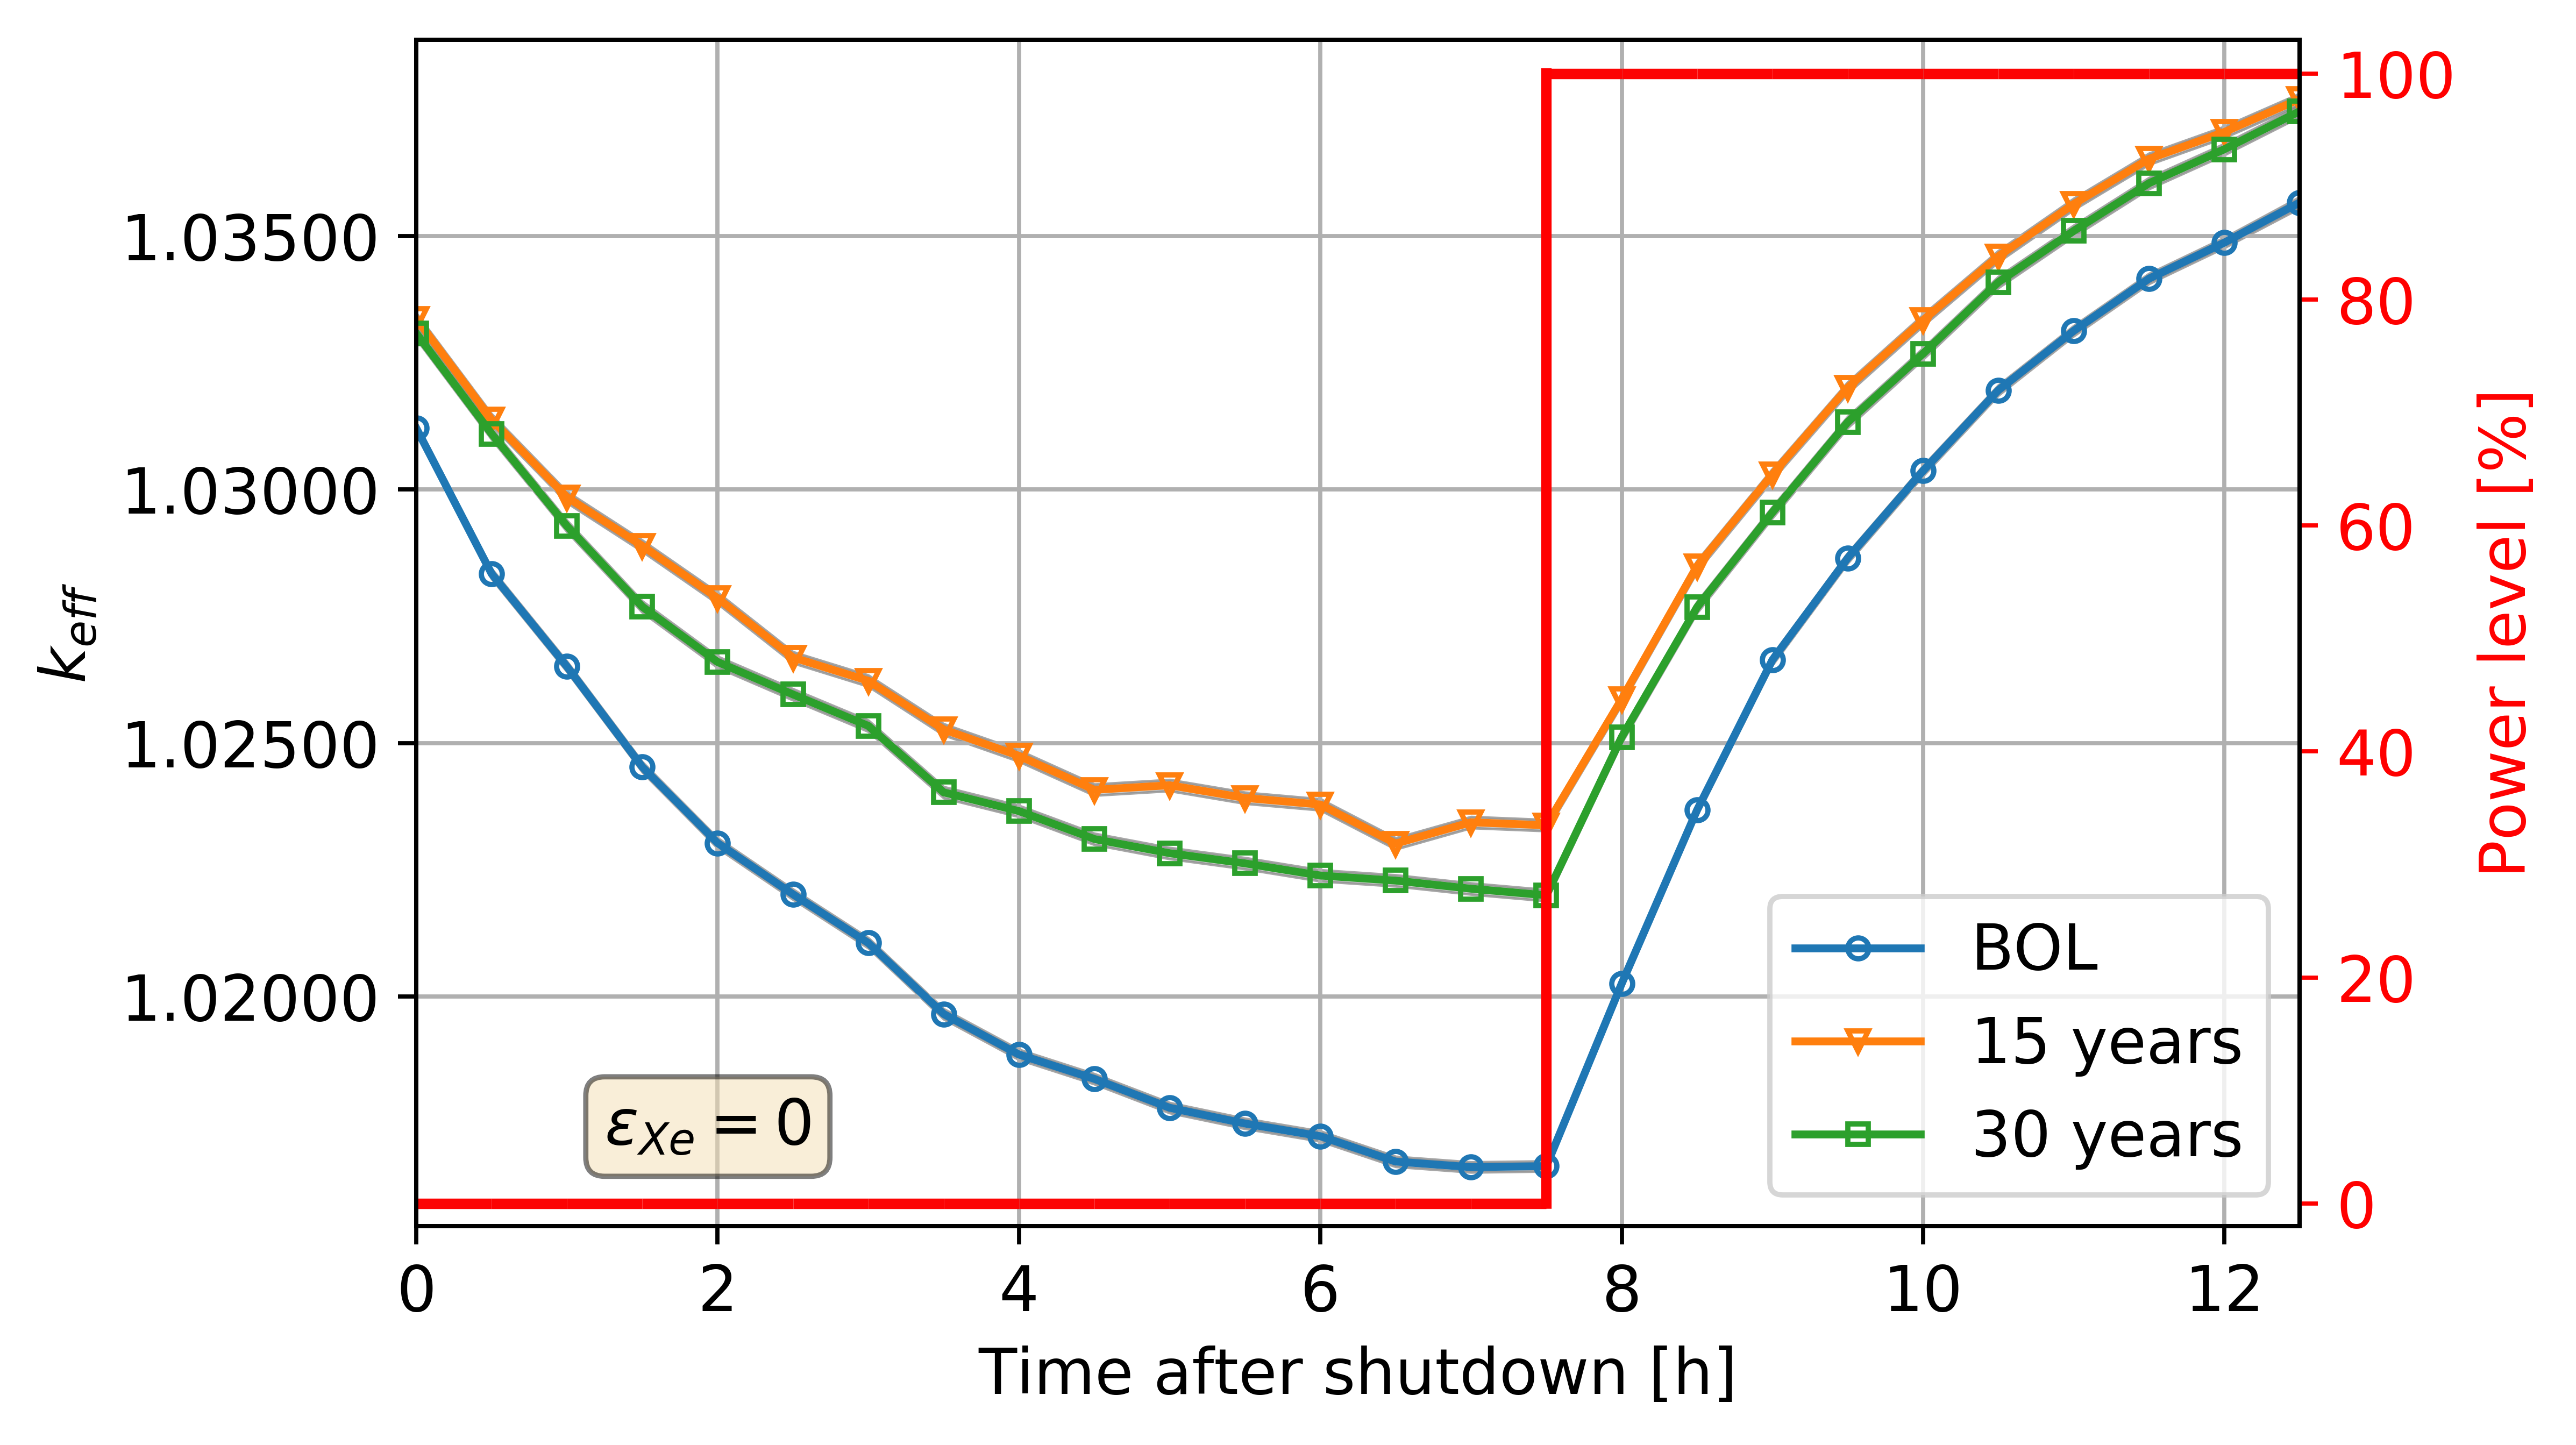
\includegraphics[width=0.92\textwidth]{ch6/kl1_keff.png}\vspace{-14mm}\\
	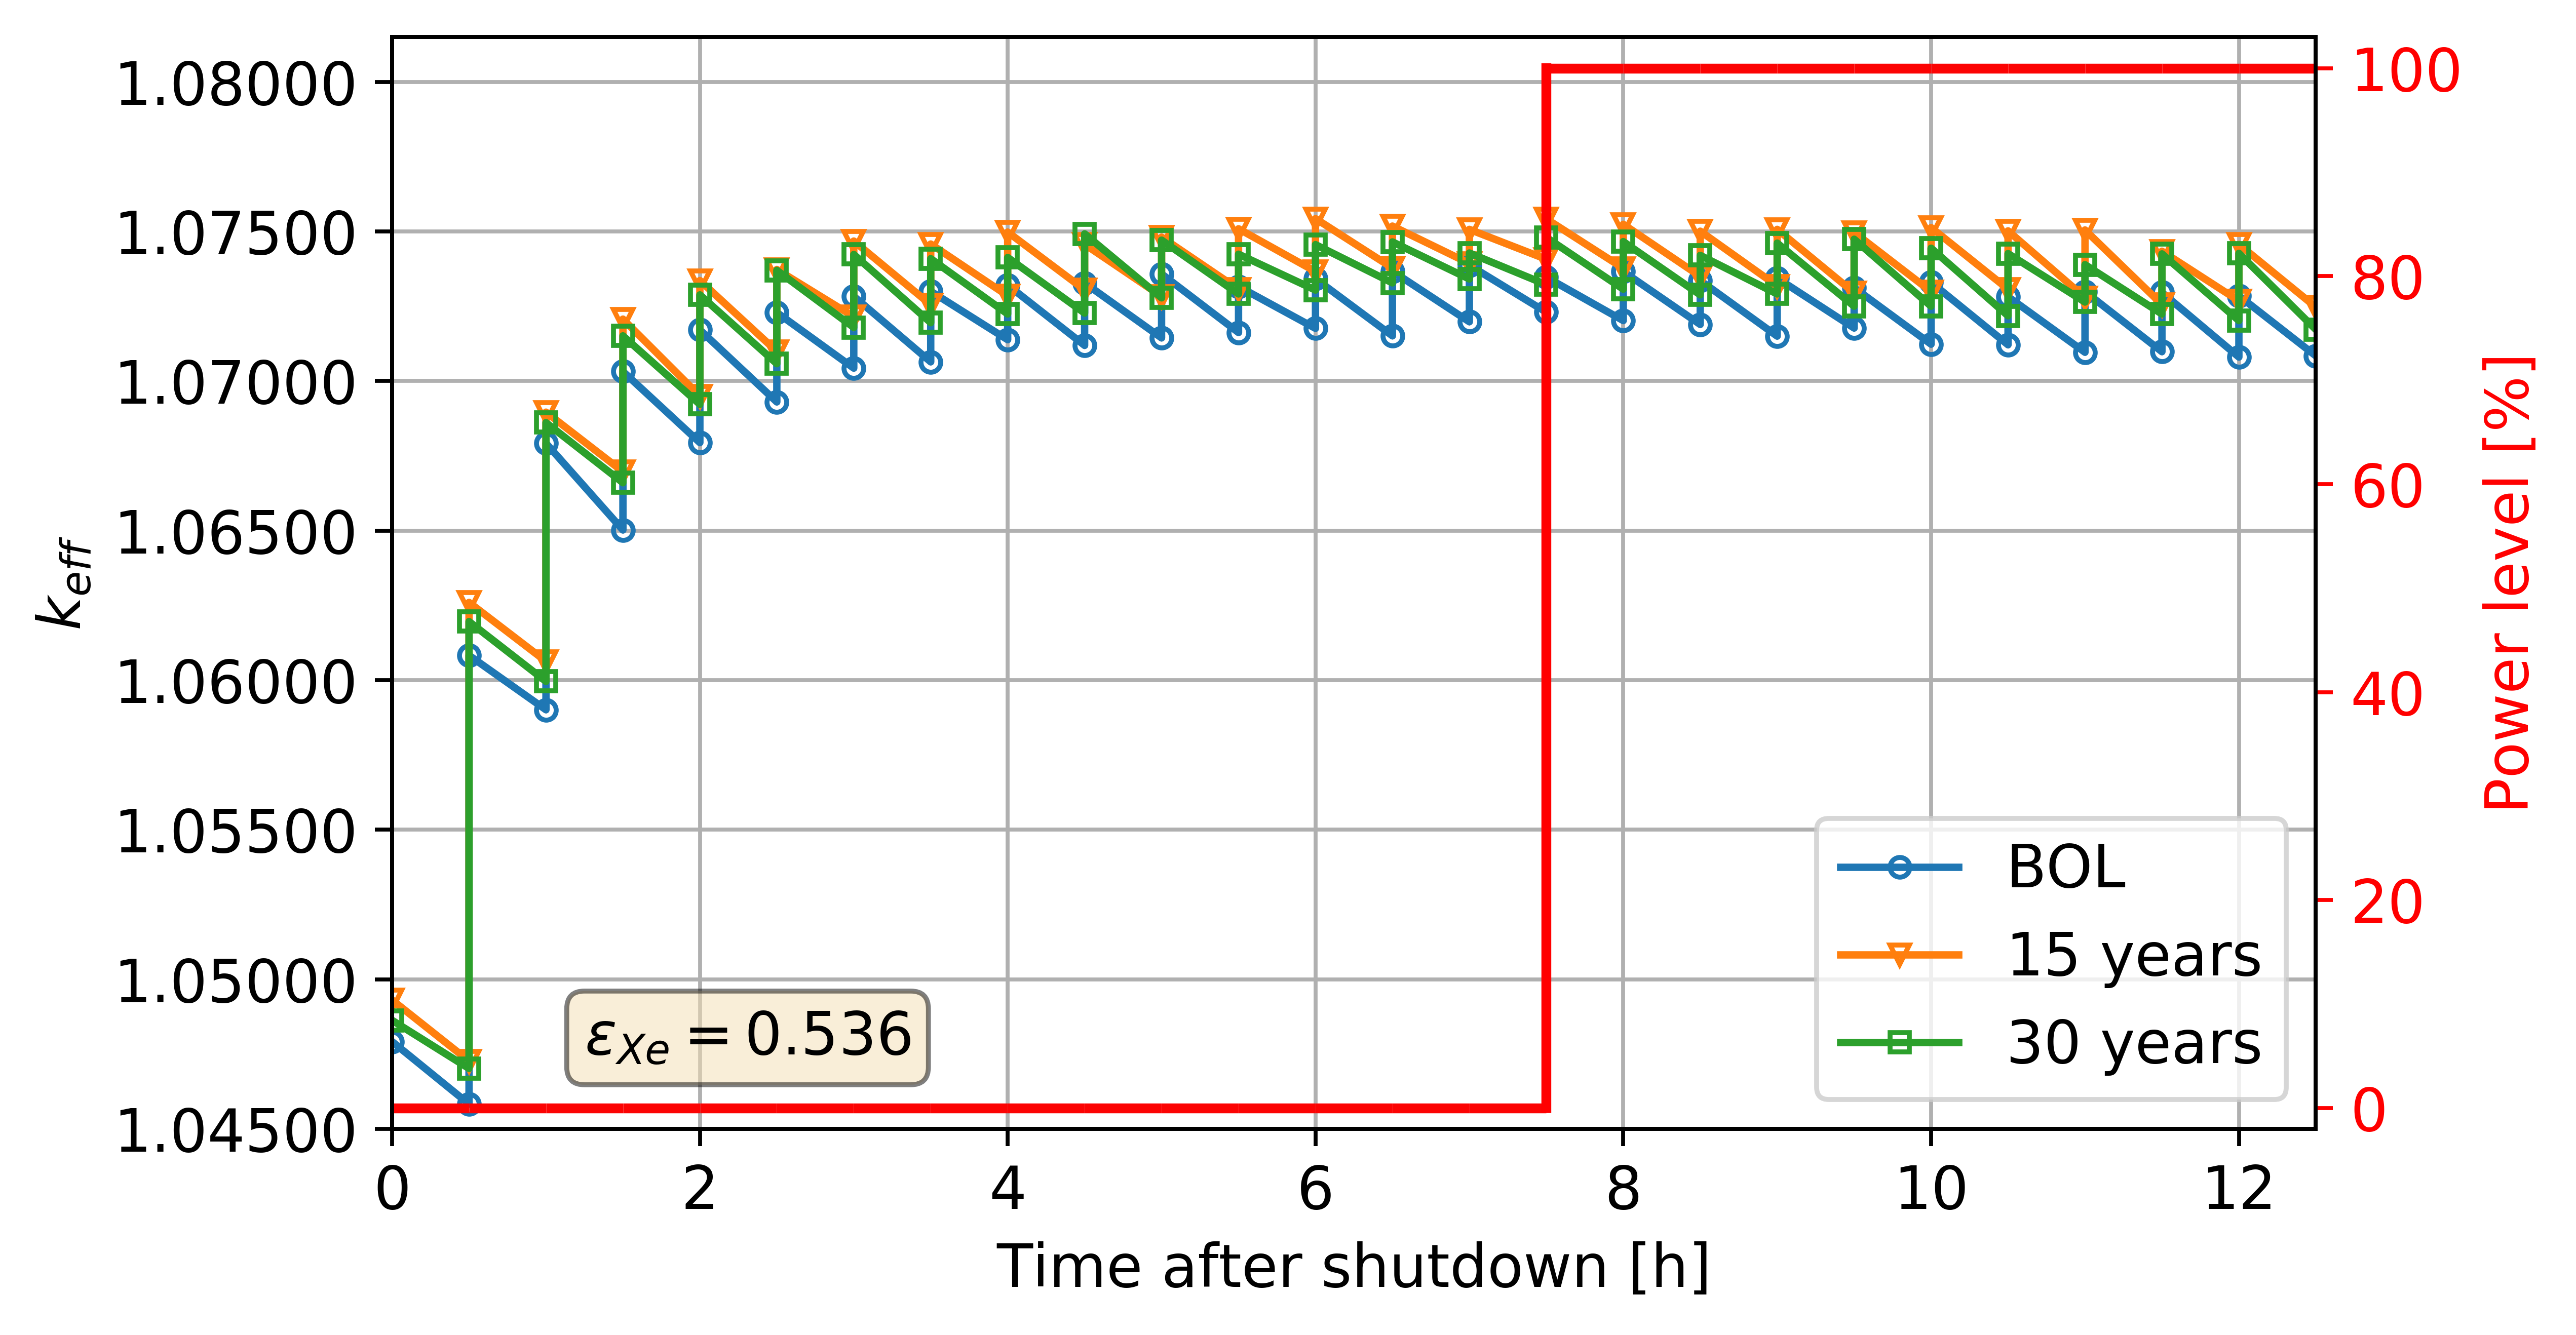
\includegraphics[width=0.905\textwidth]{ch6/kl25_keff.png}\vspace{-12mm}\\
	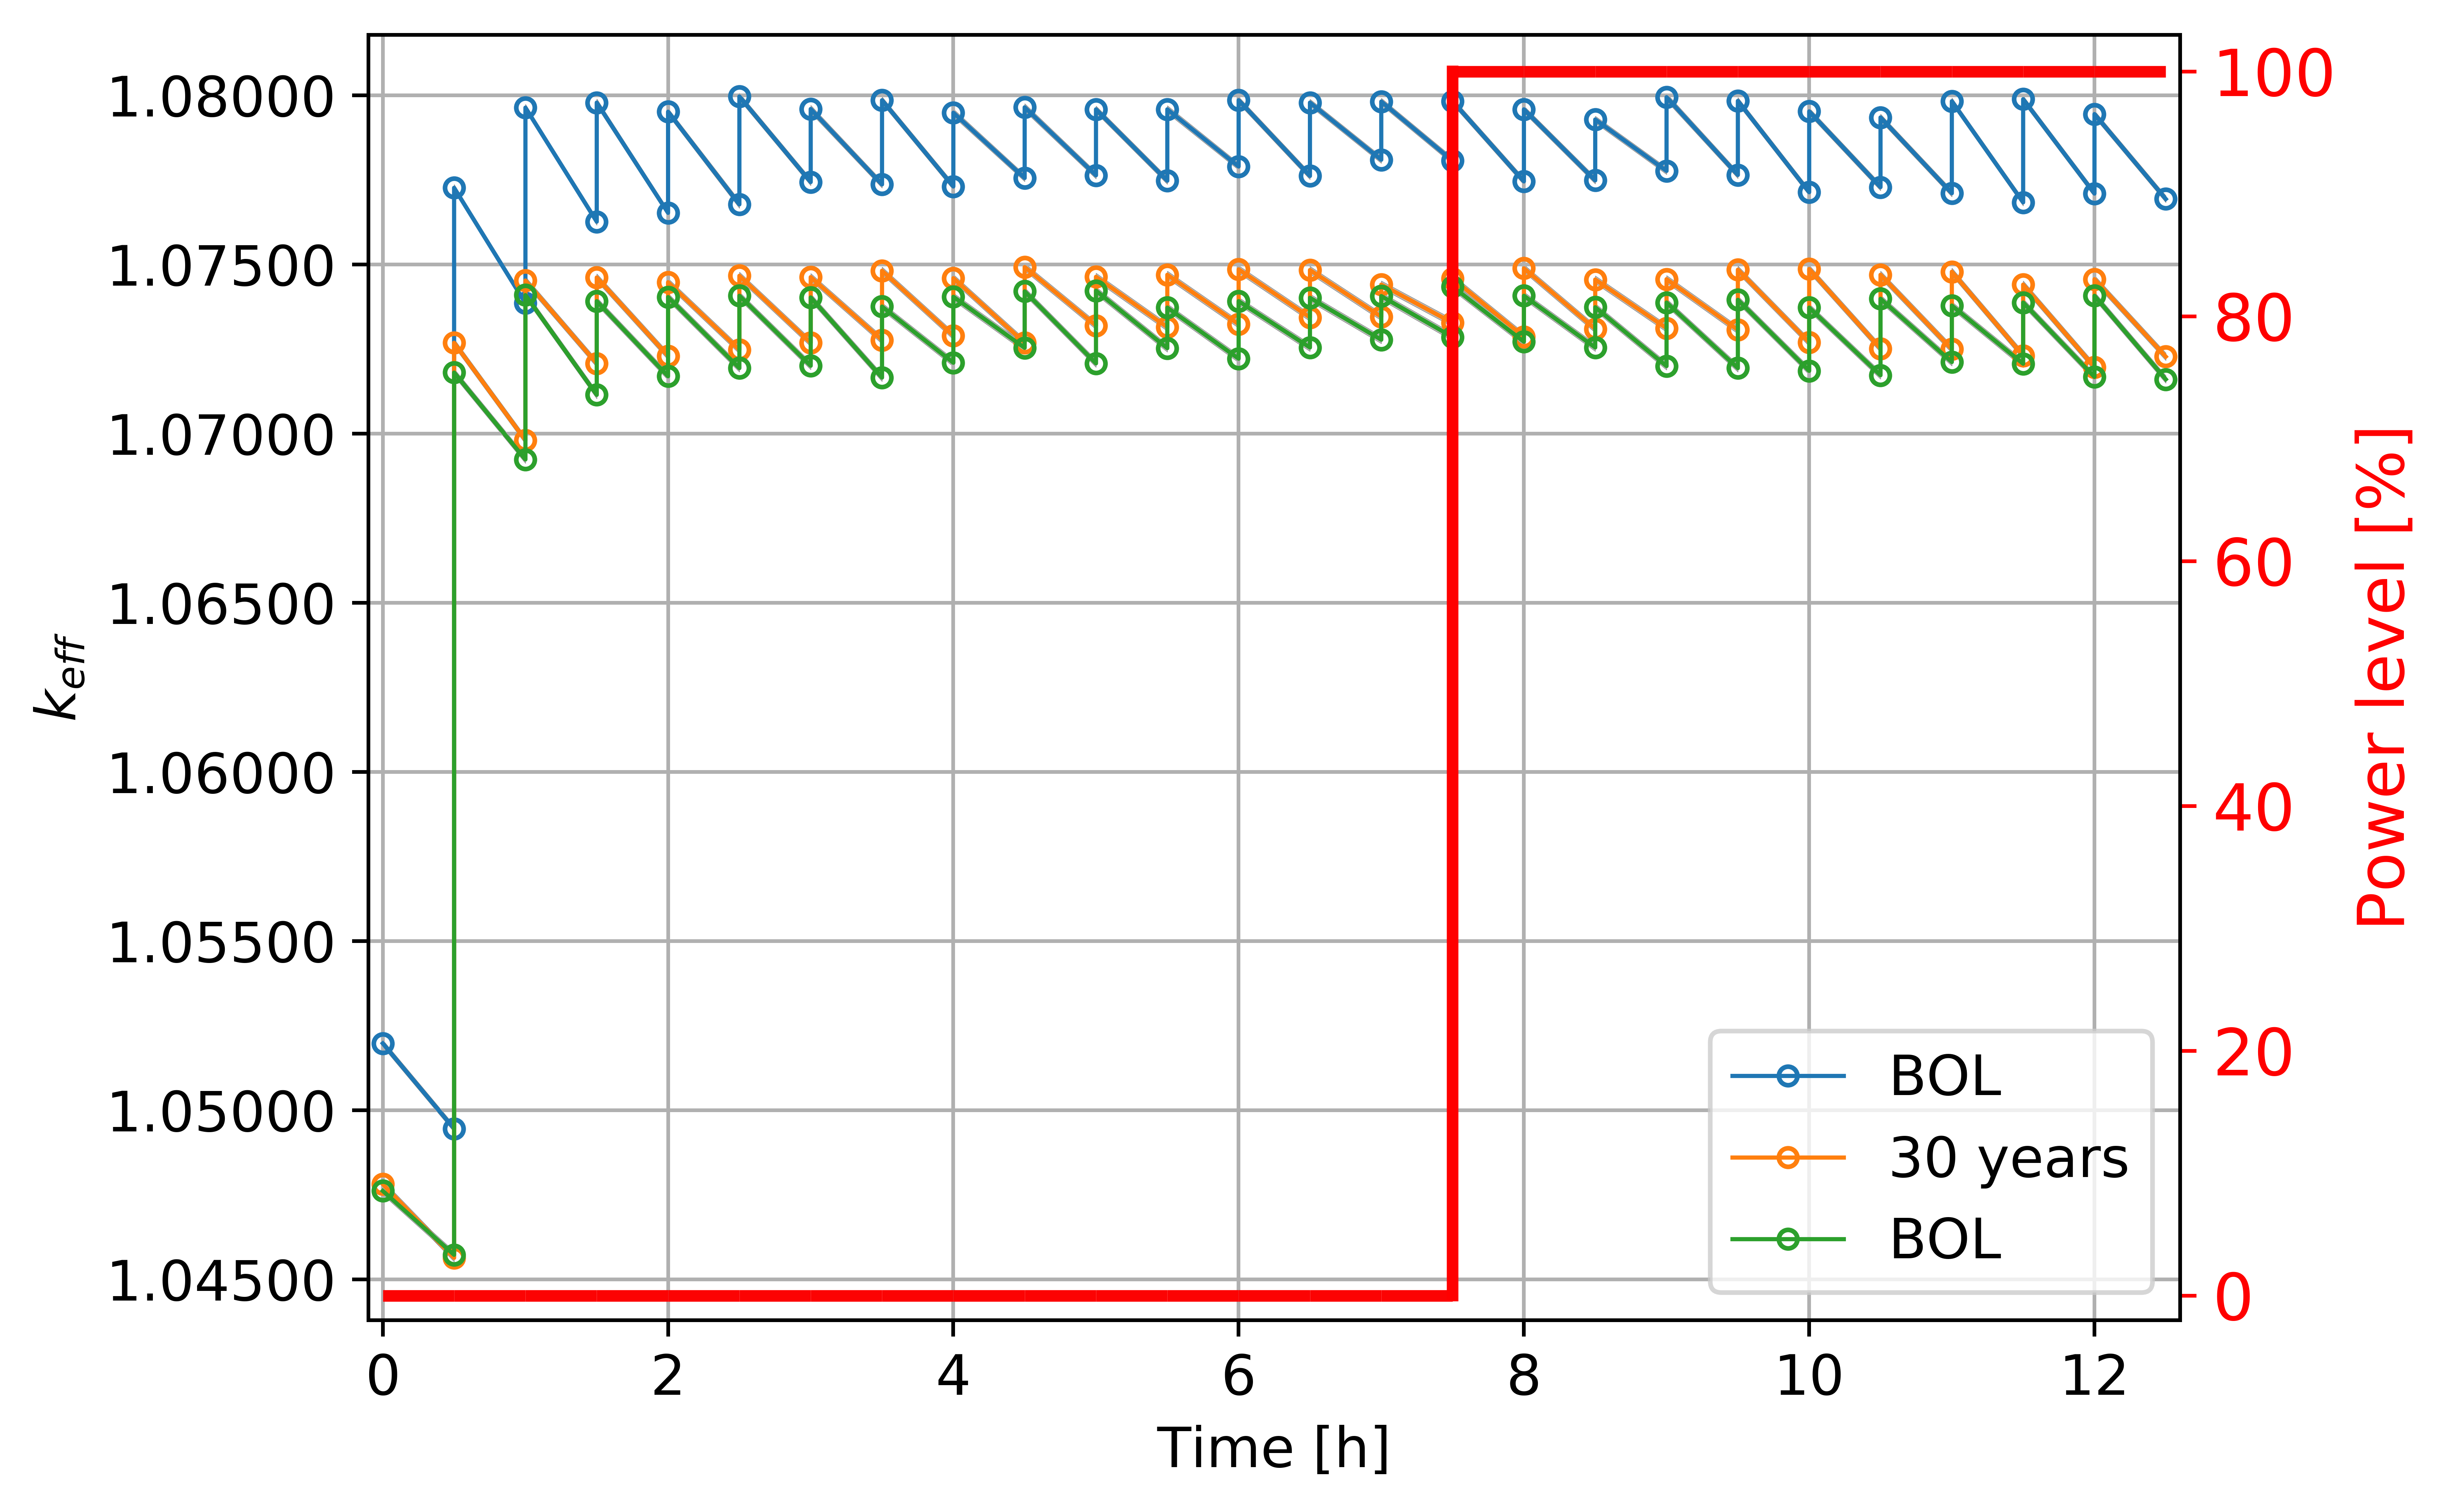
\includegraphics[width=0.905\textwidth]{ch6/kl100_keff.png}
\end{array}$
		\vspace{-5mm}
	\caption{SaltProc-calculated evolution of the effective multiplication 
	factor during the postulated load-following transient for various regimes 
	of the gas removal system operation. The uncertainty $\pm\sigma=10$ $pcm$ 
	is shaded.}
	\label{fig:msbr-lf-keff-evo}
\end{figure}

\begin{figure}[htbp!] % replace 't' with 'b' to 
	\centering
	$\begin{array}{r}
	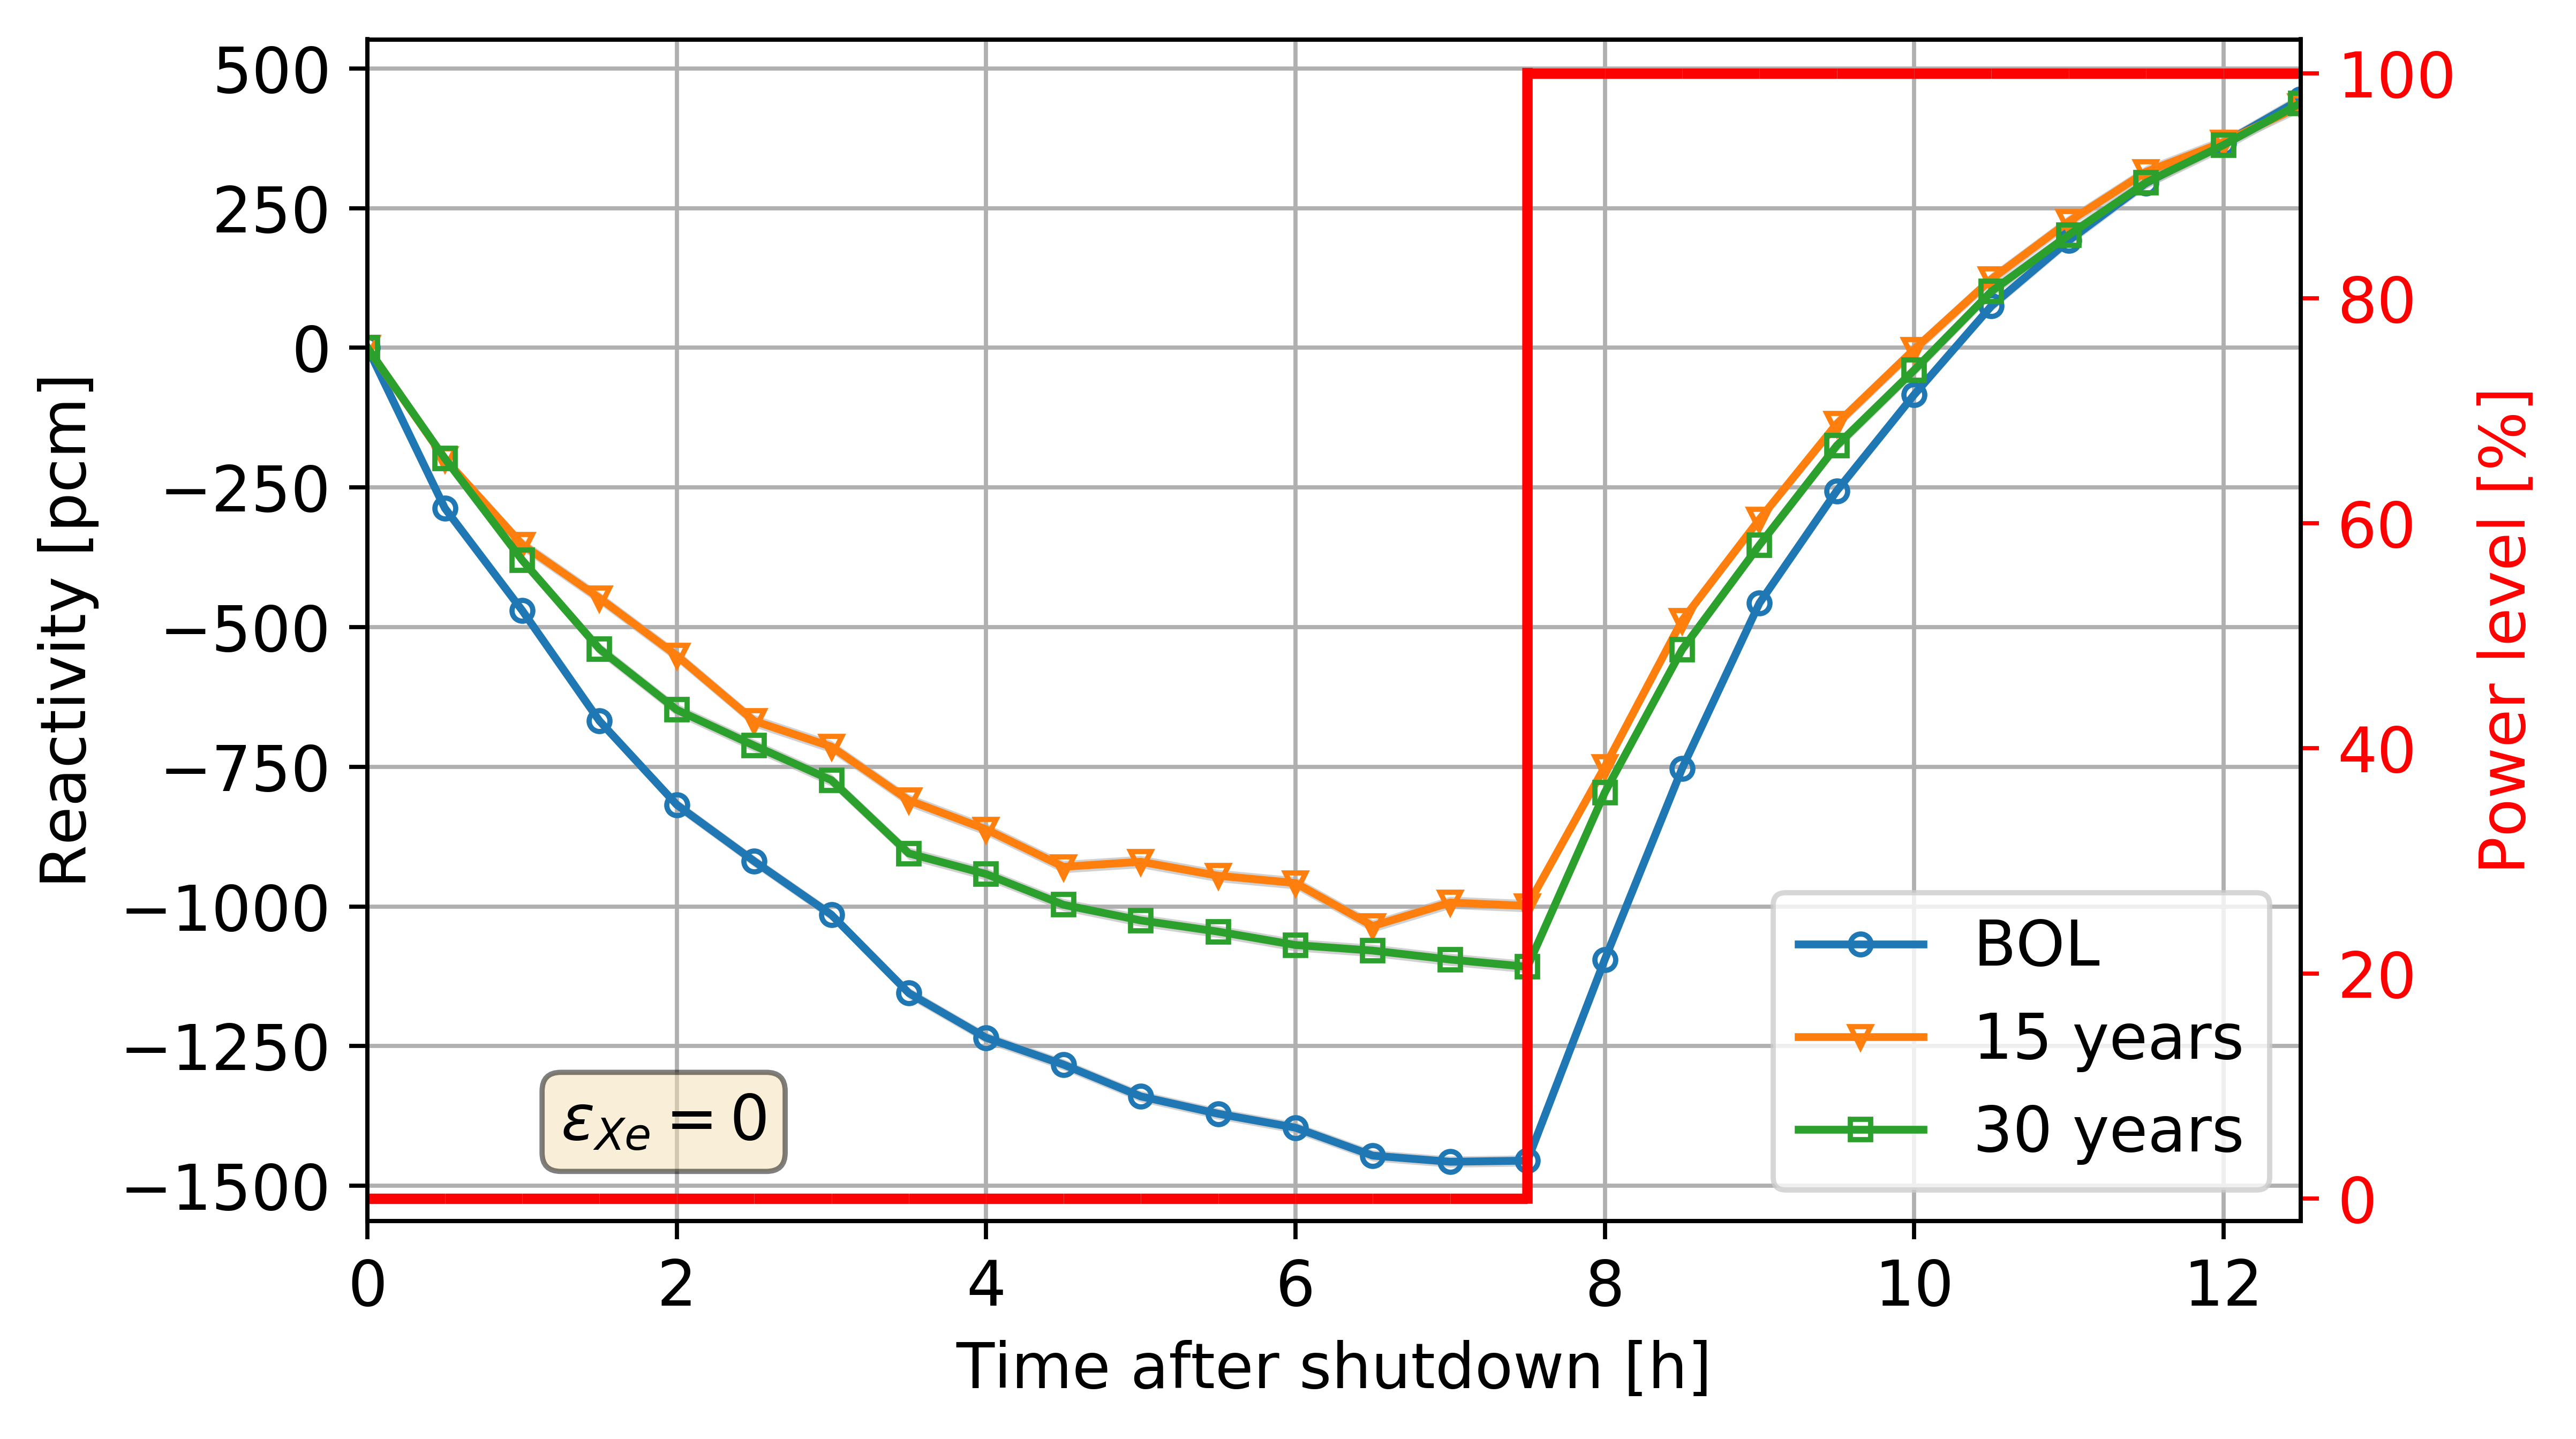
\includegraphics[width=0.923\textwidth]{ch6/kl1_rho.png}\vspace{-14mm}\\
	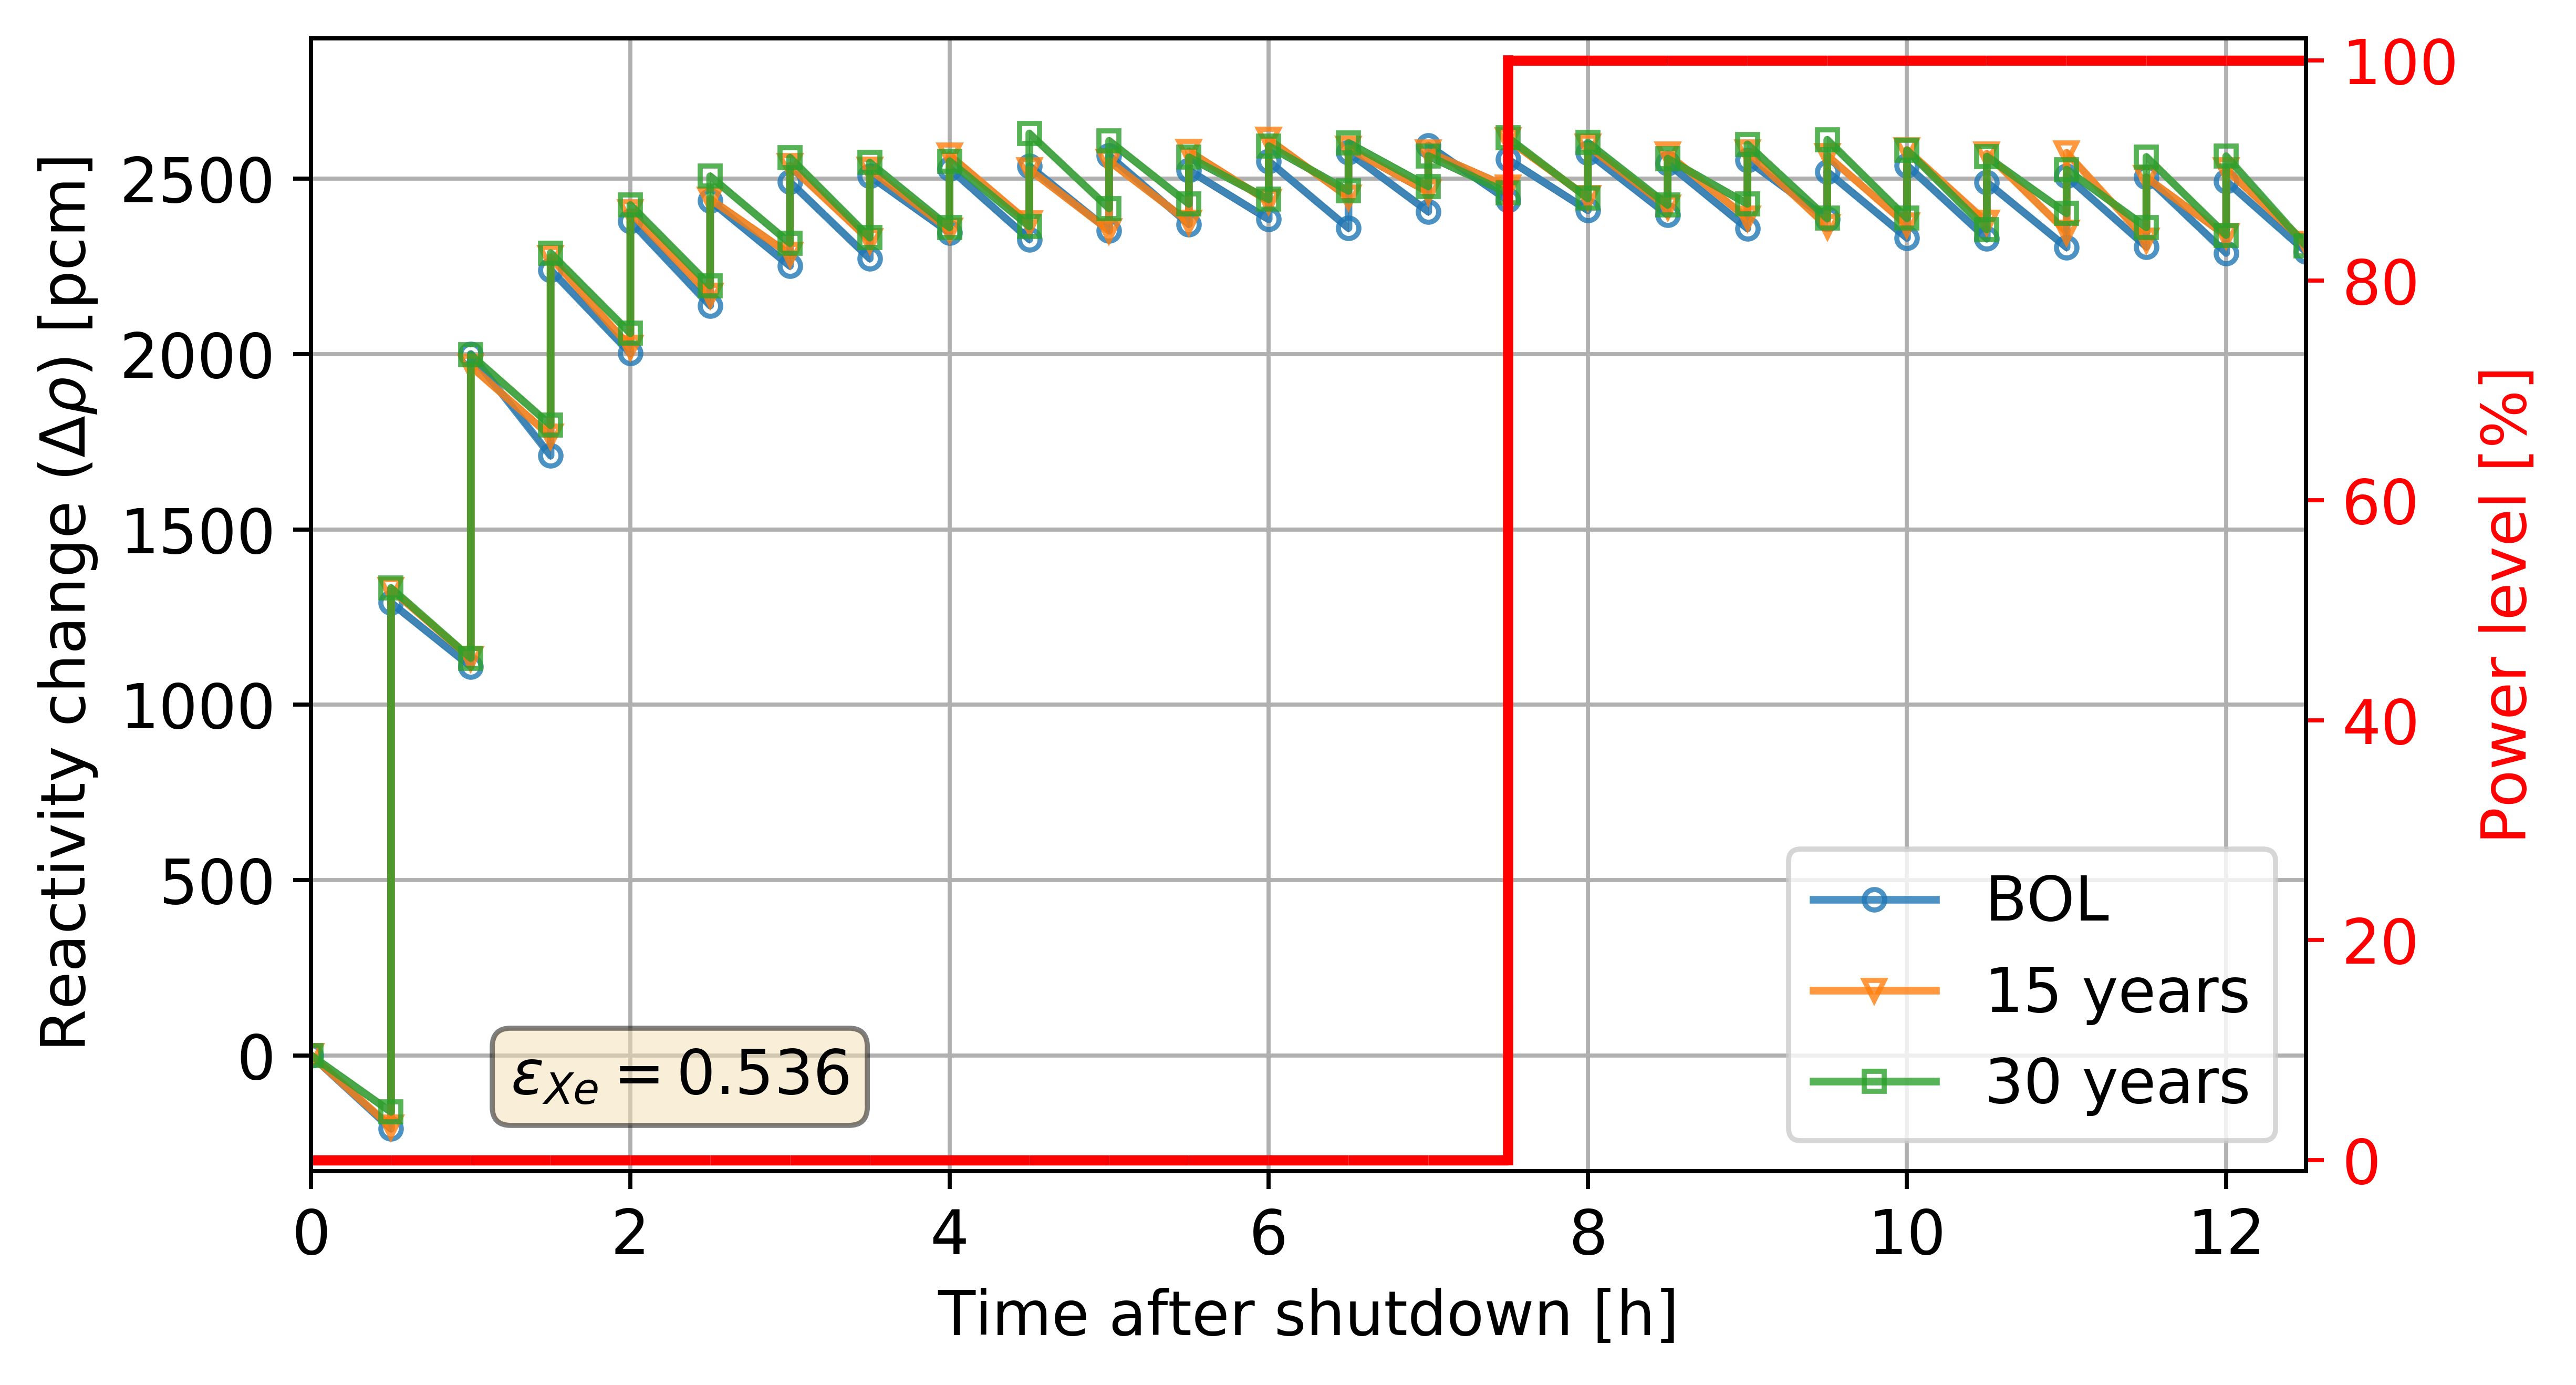
\includegraphics[width=0.9\textwidth]{ch6/kl25_rho.png}\vspace{-13mm}\\
	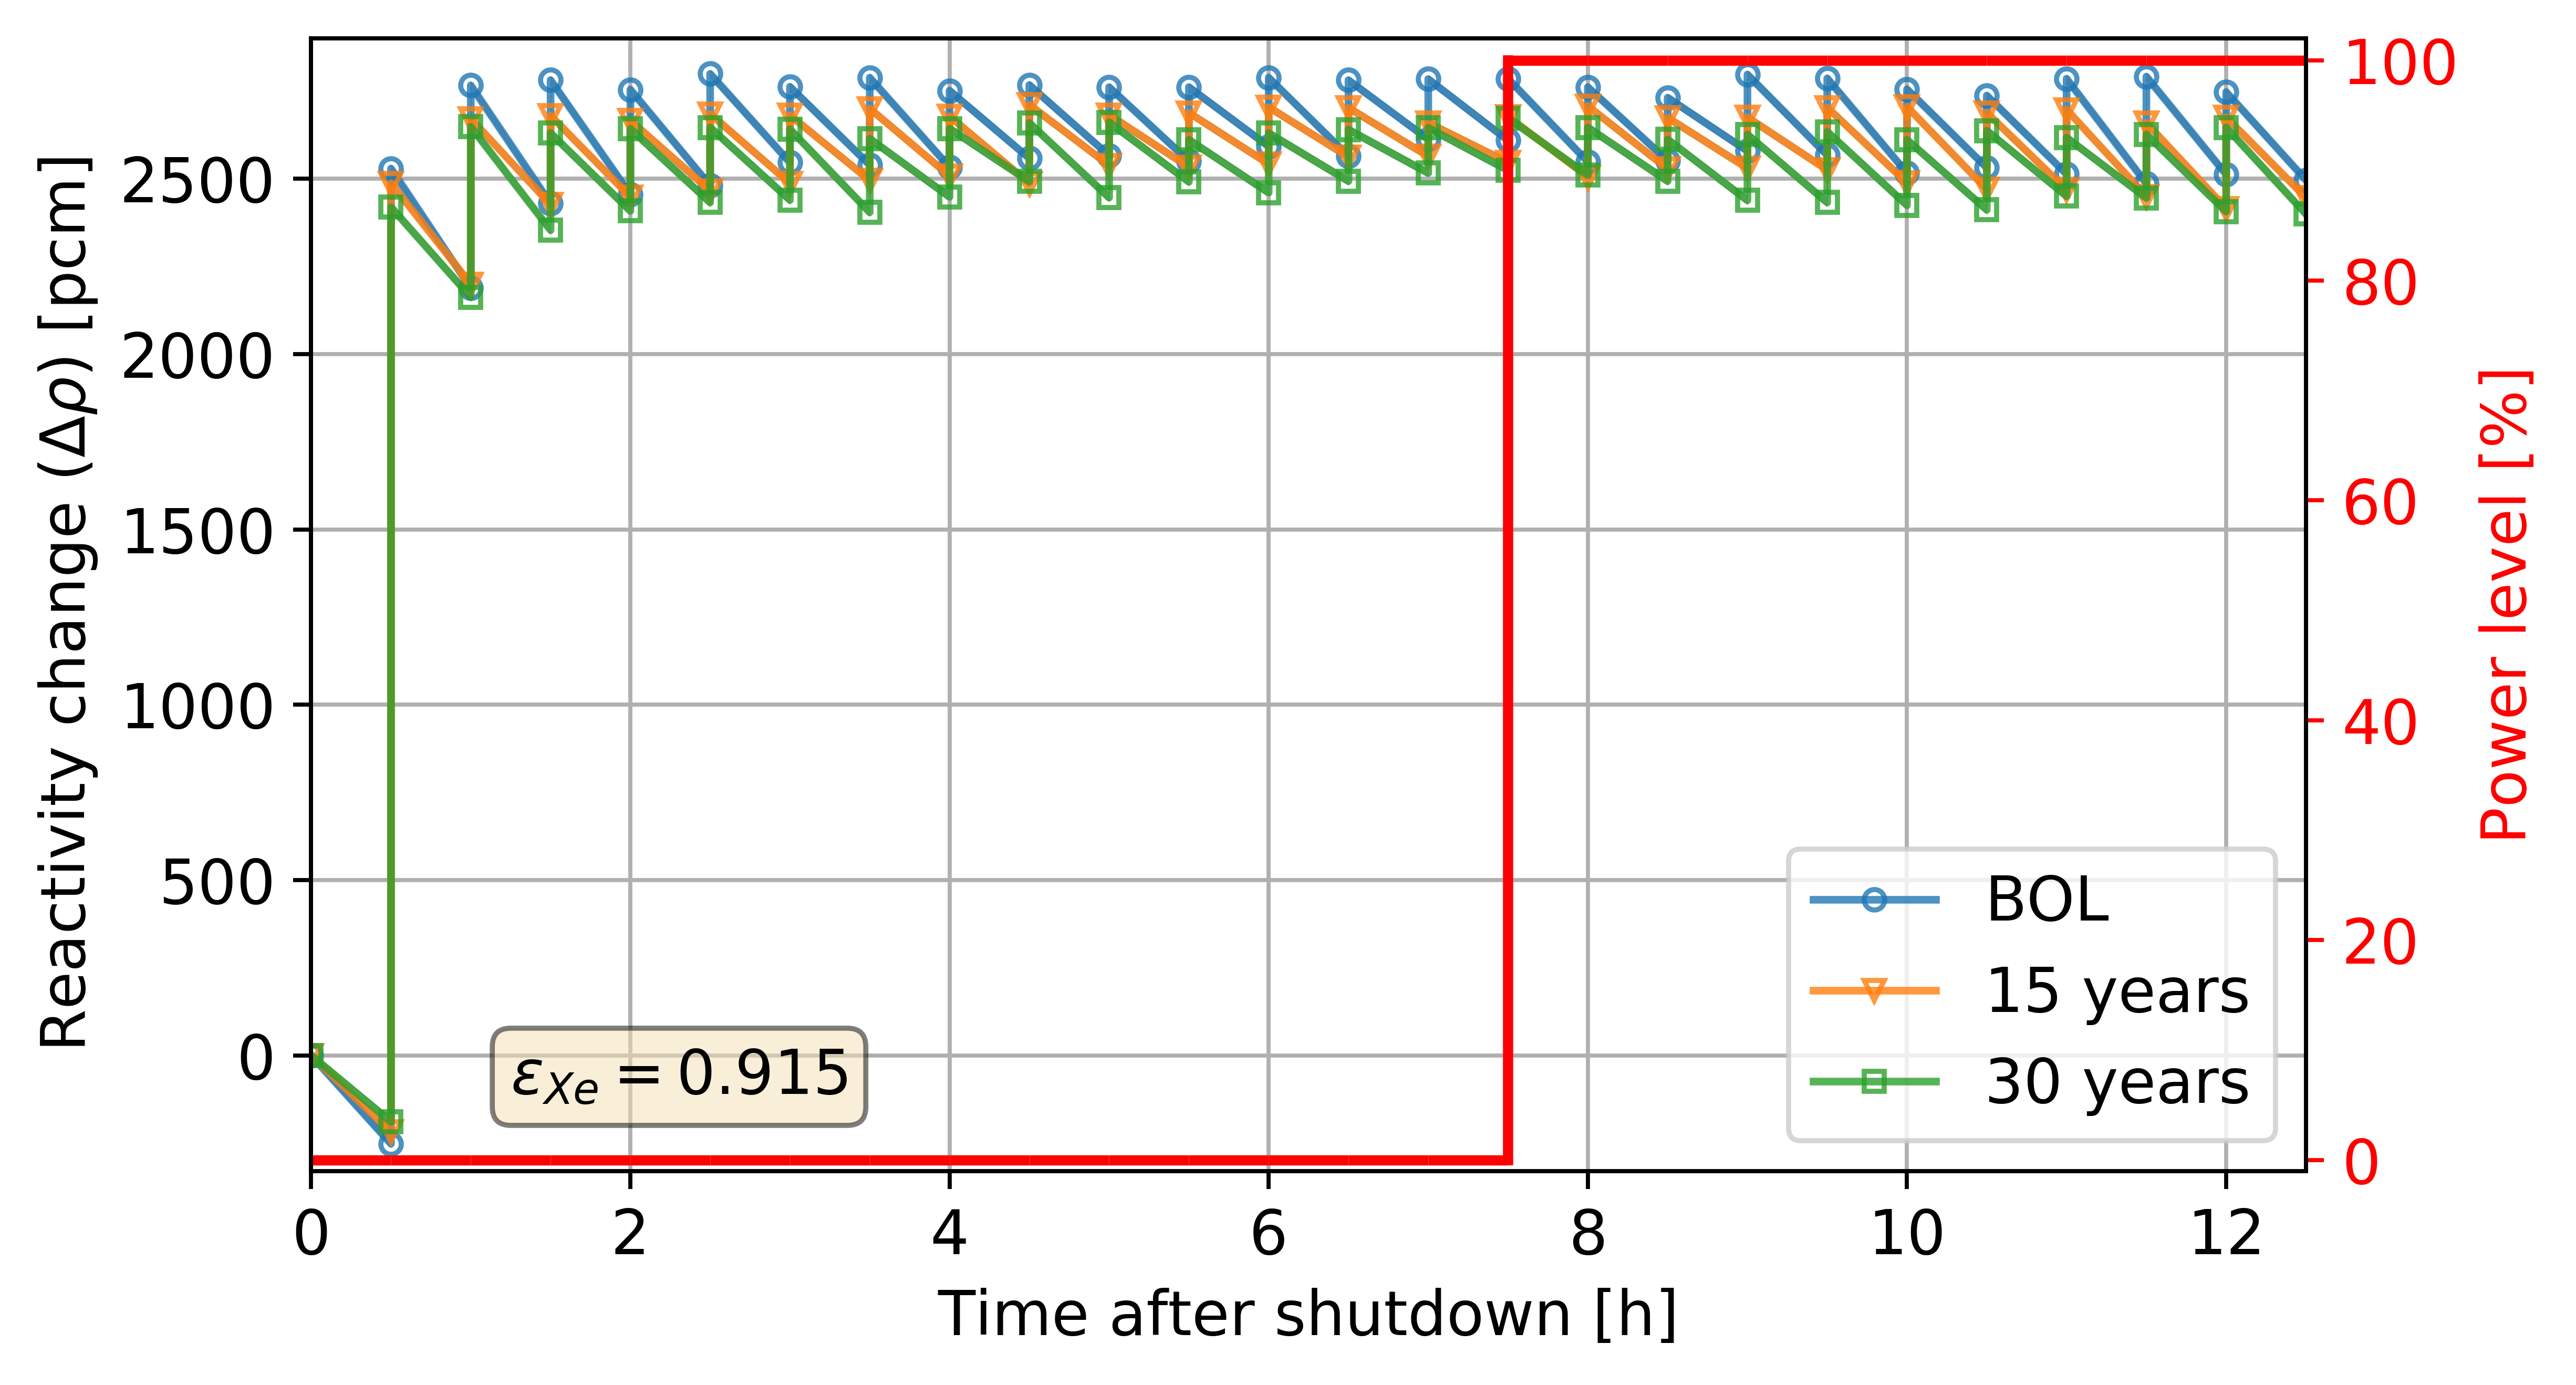
\includegraphics[width=0.9\textwidth]{ch6/kl100_rho.png}
	\end{array}$
	\vspace{-5mm}
	\caption{SaltProc-calculated evolution of the reactivity during the 
	postulated load-following transient for various regimes 
		of the gas removal system operation. The uncertainty $\pm\sigma=10$ 
		$pcm$ 
		is shaded.}
	\label{fig:msbr-lf-rho-evo}
\end{figure}
\FloatBarrier

\subsection{Fuel salt composition evolution}
Figure~\ref{fig:msbr-lf-xe-i-ratio} shows $^{135}$Xe and $^{135}$I mass 
dynamics evolution during the postulated transient for various gas removal 
efficiencies. The $^{135}$I/$^{135}$Xe concentration ratio at the beginning 
transient for the no-removal case is 2.45 and 2.03 at the \gls{BOL} and after 
30 years of full-power operation, respectively. The greater 
$^{135}$I/$^{135}$Xe concentration ratio at the startup leads to $^{135}$Xe 
concentration peak by 11\% higher than at the \gls{EOL} which is consistent 
with the \gls{TAP} \gls{MSR} results. However, larger $^{135}$Xe concentration 
does not worsen the xenon poisoning effect (Figure~\ref{fig:msbr-lf-rho-evo}) 
because the spectrum hardens toward \gls{EOL}. The harder spectrum leads to 
weaker $^{135}$Xe burn out because its absorption cross section slumps with 
energy (see Figure~\ref{fig:tap-pwr-spectrum}).

For the high gas removal efficiency regime, the $^{135}$I/$^{135}$Xe 
concentration ratio is 2.47 and 2.08 at the \gls{BOL} and after 
30 years of full-power operation, respectively. For the \gls{BOL} and 
\gls{EOL}, the $^{135}$Xe concentration peaked only by 8\% at the end of first 
30-minute depletion step which caused a 189-$pcm$ negative reactivity 
insertion. Afterward, the concentration of $^{135}$Xe dropped quickly because 
the gas removal system extracted most of the fission gas. The mass of 
$^{135}$Xe in the fuel salt before shutdown is approximately 7 times greater 
than after the power turned back on, which caused significant reactivity 
growth by $\approx2550$ $pcm$. Surprisingly, the removal of 12 g of $^{135}$Xe 
after 60 minutes from the shutdown caused an impressive 2600-$pcm$ positive 
reactivity insertion (217 pcm/g$^{135}$Xe reactivity worth). 
\begin{figure}[htbp!] % replace 't' with 'b' to 
	\centering
	$\begin{array}{r}
	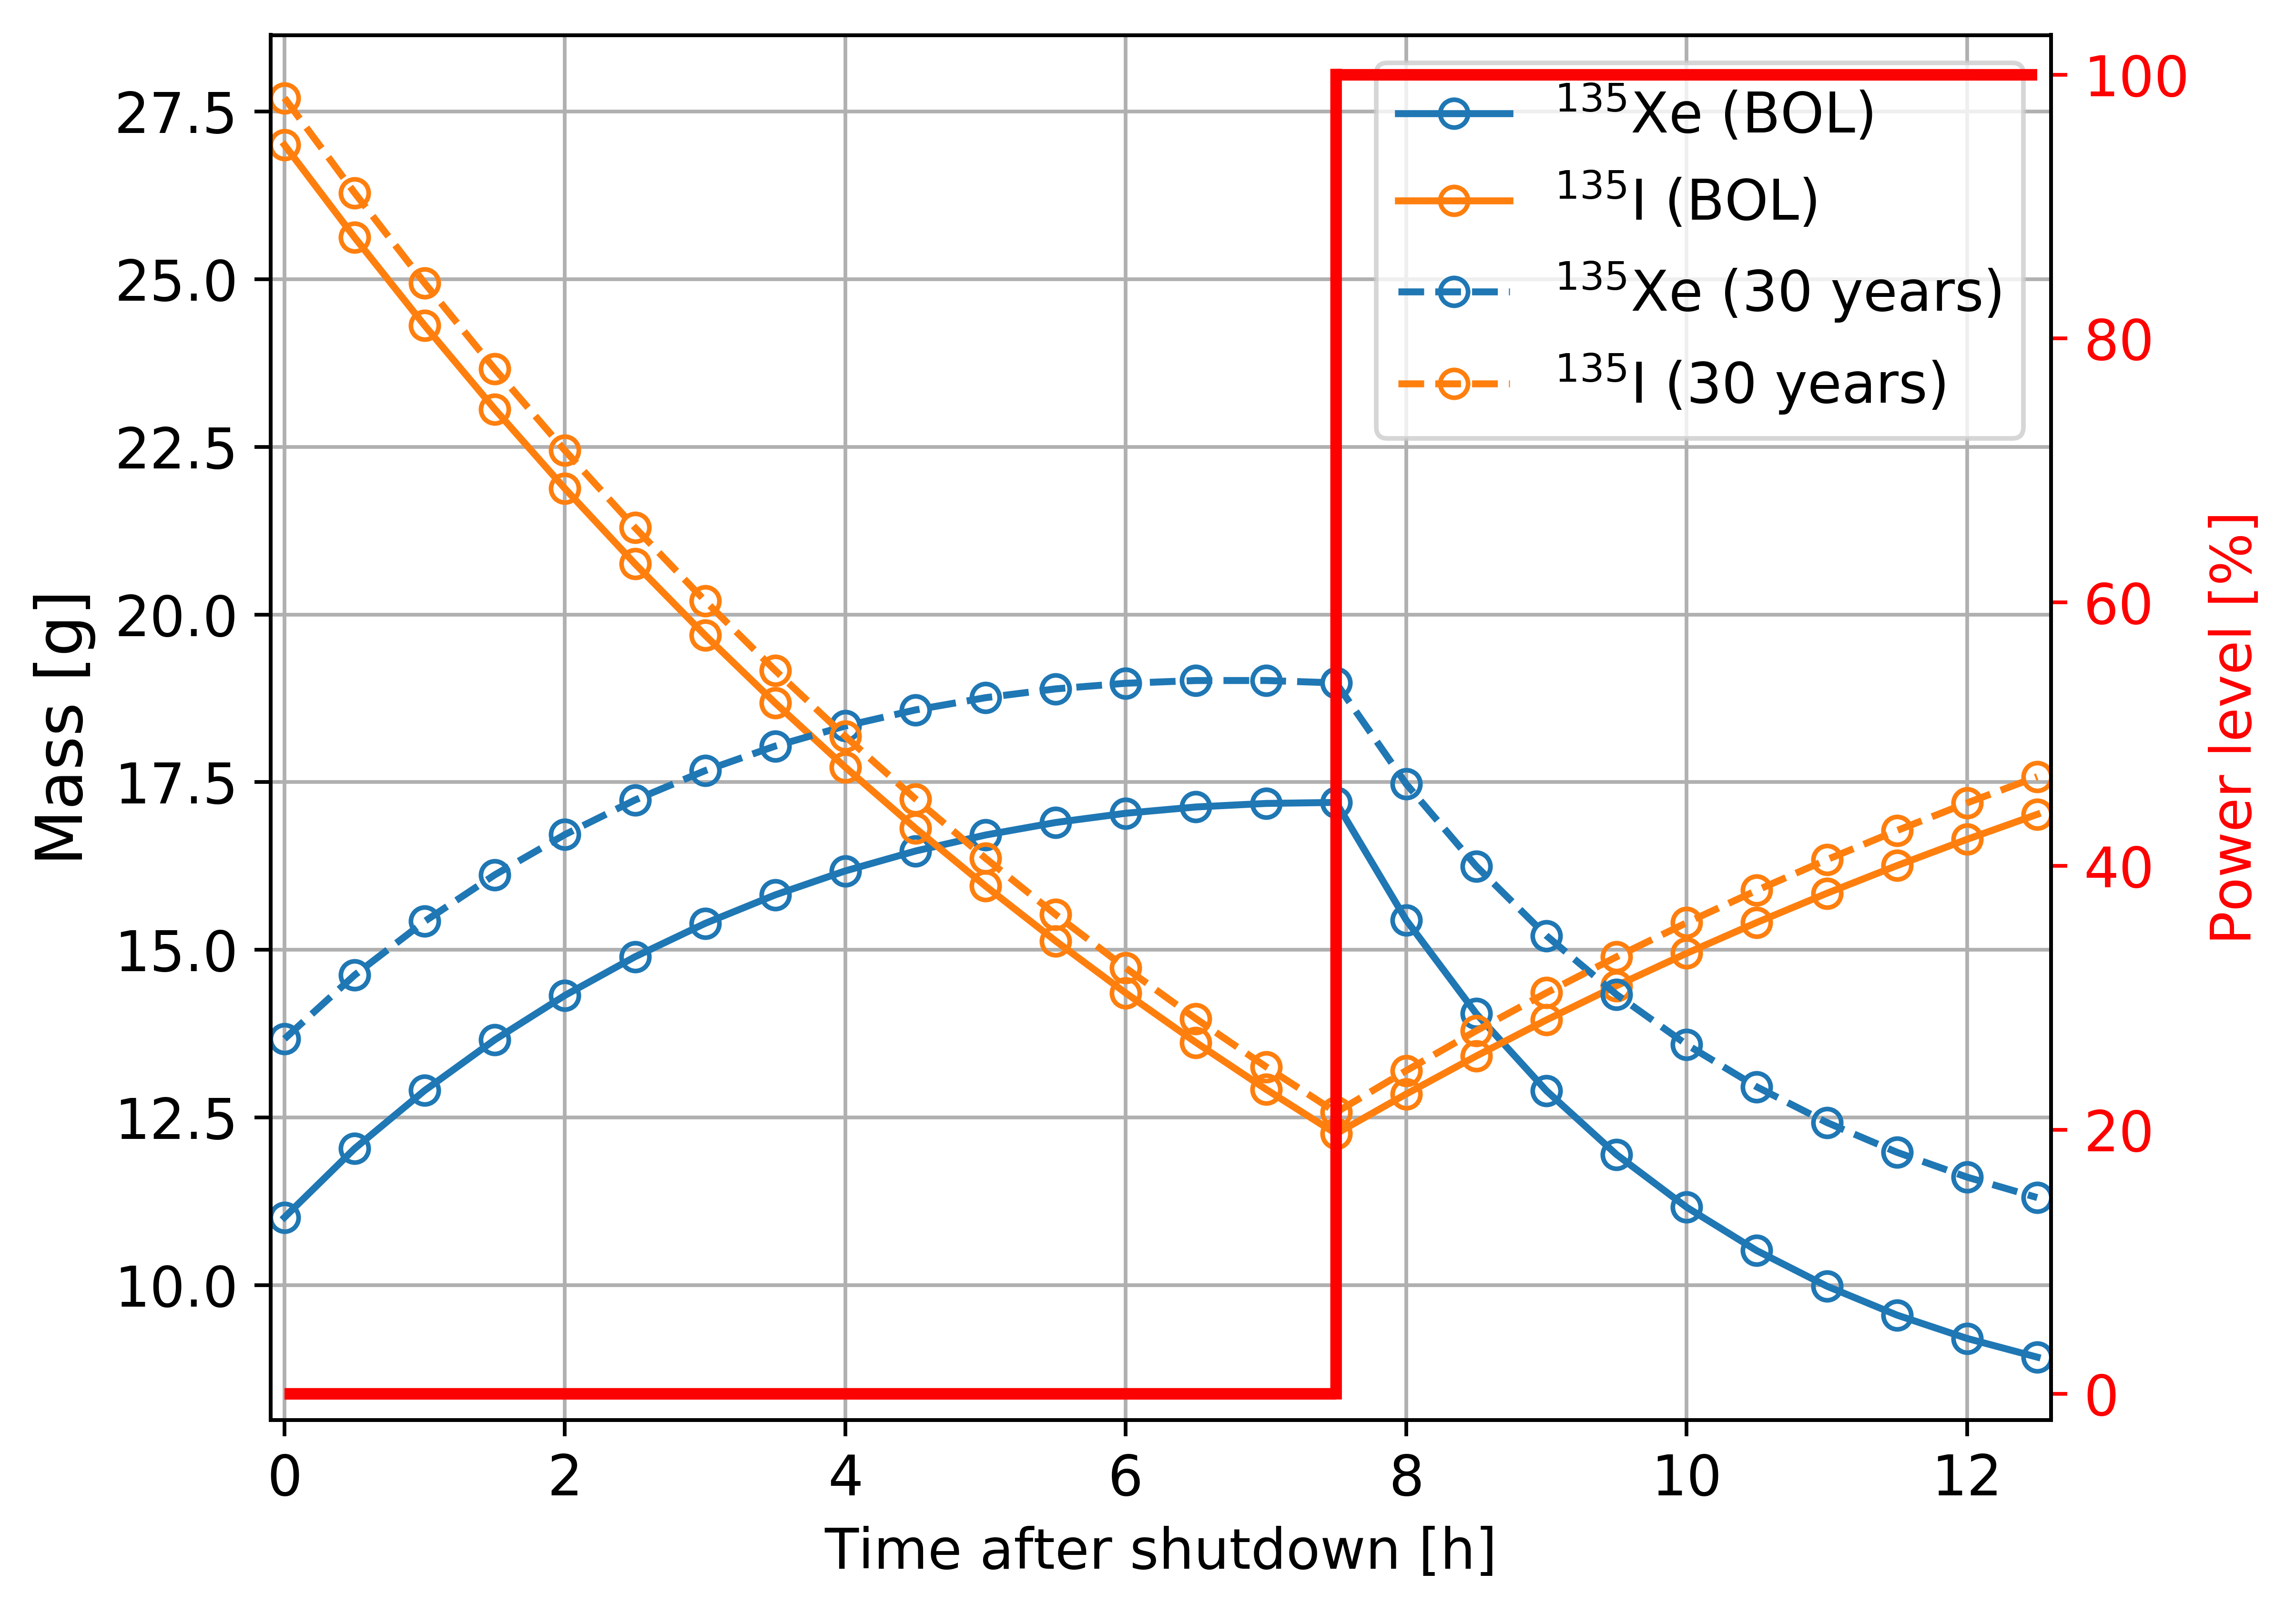
\includegraphics[width=0.88\textwidth]{ch6/kl1_xe_i_ratio.png}\vspace{-13mm}\\
	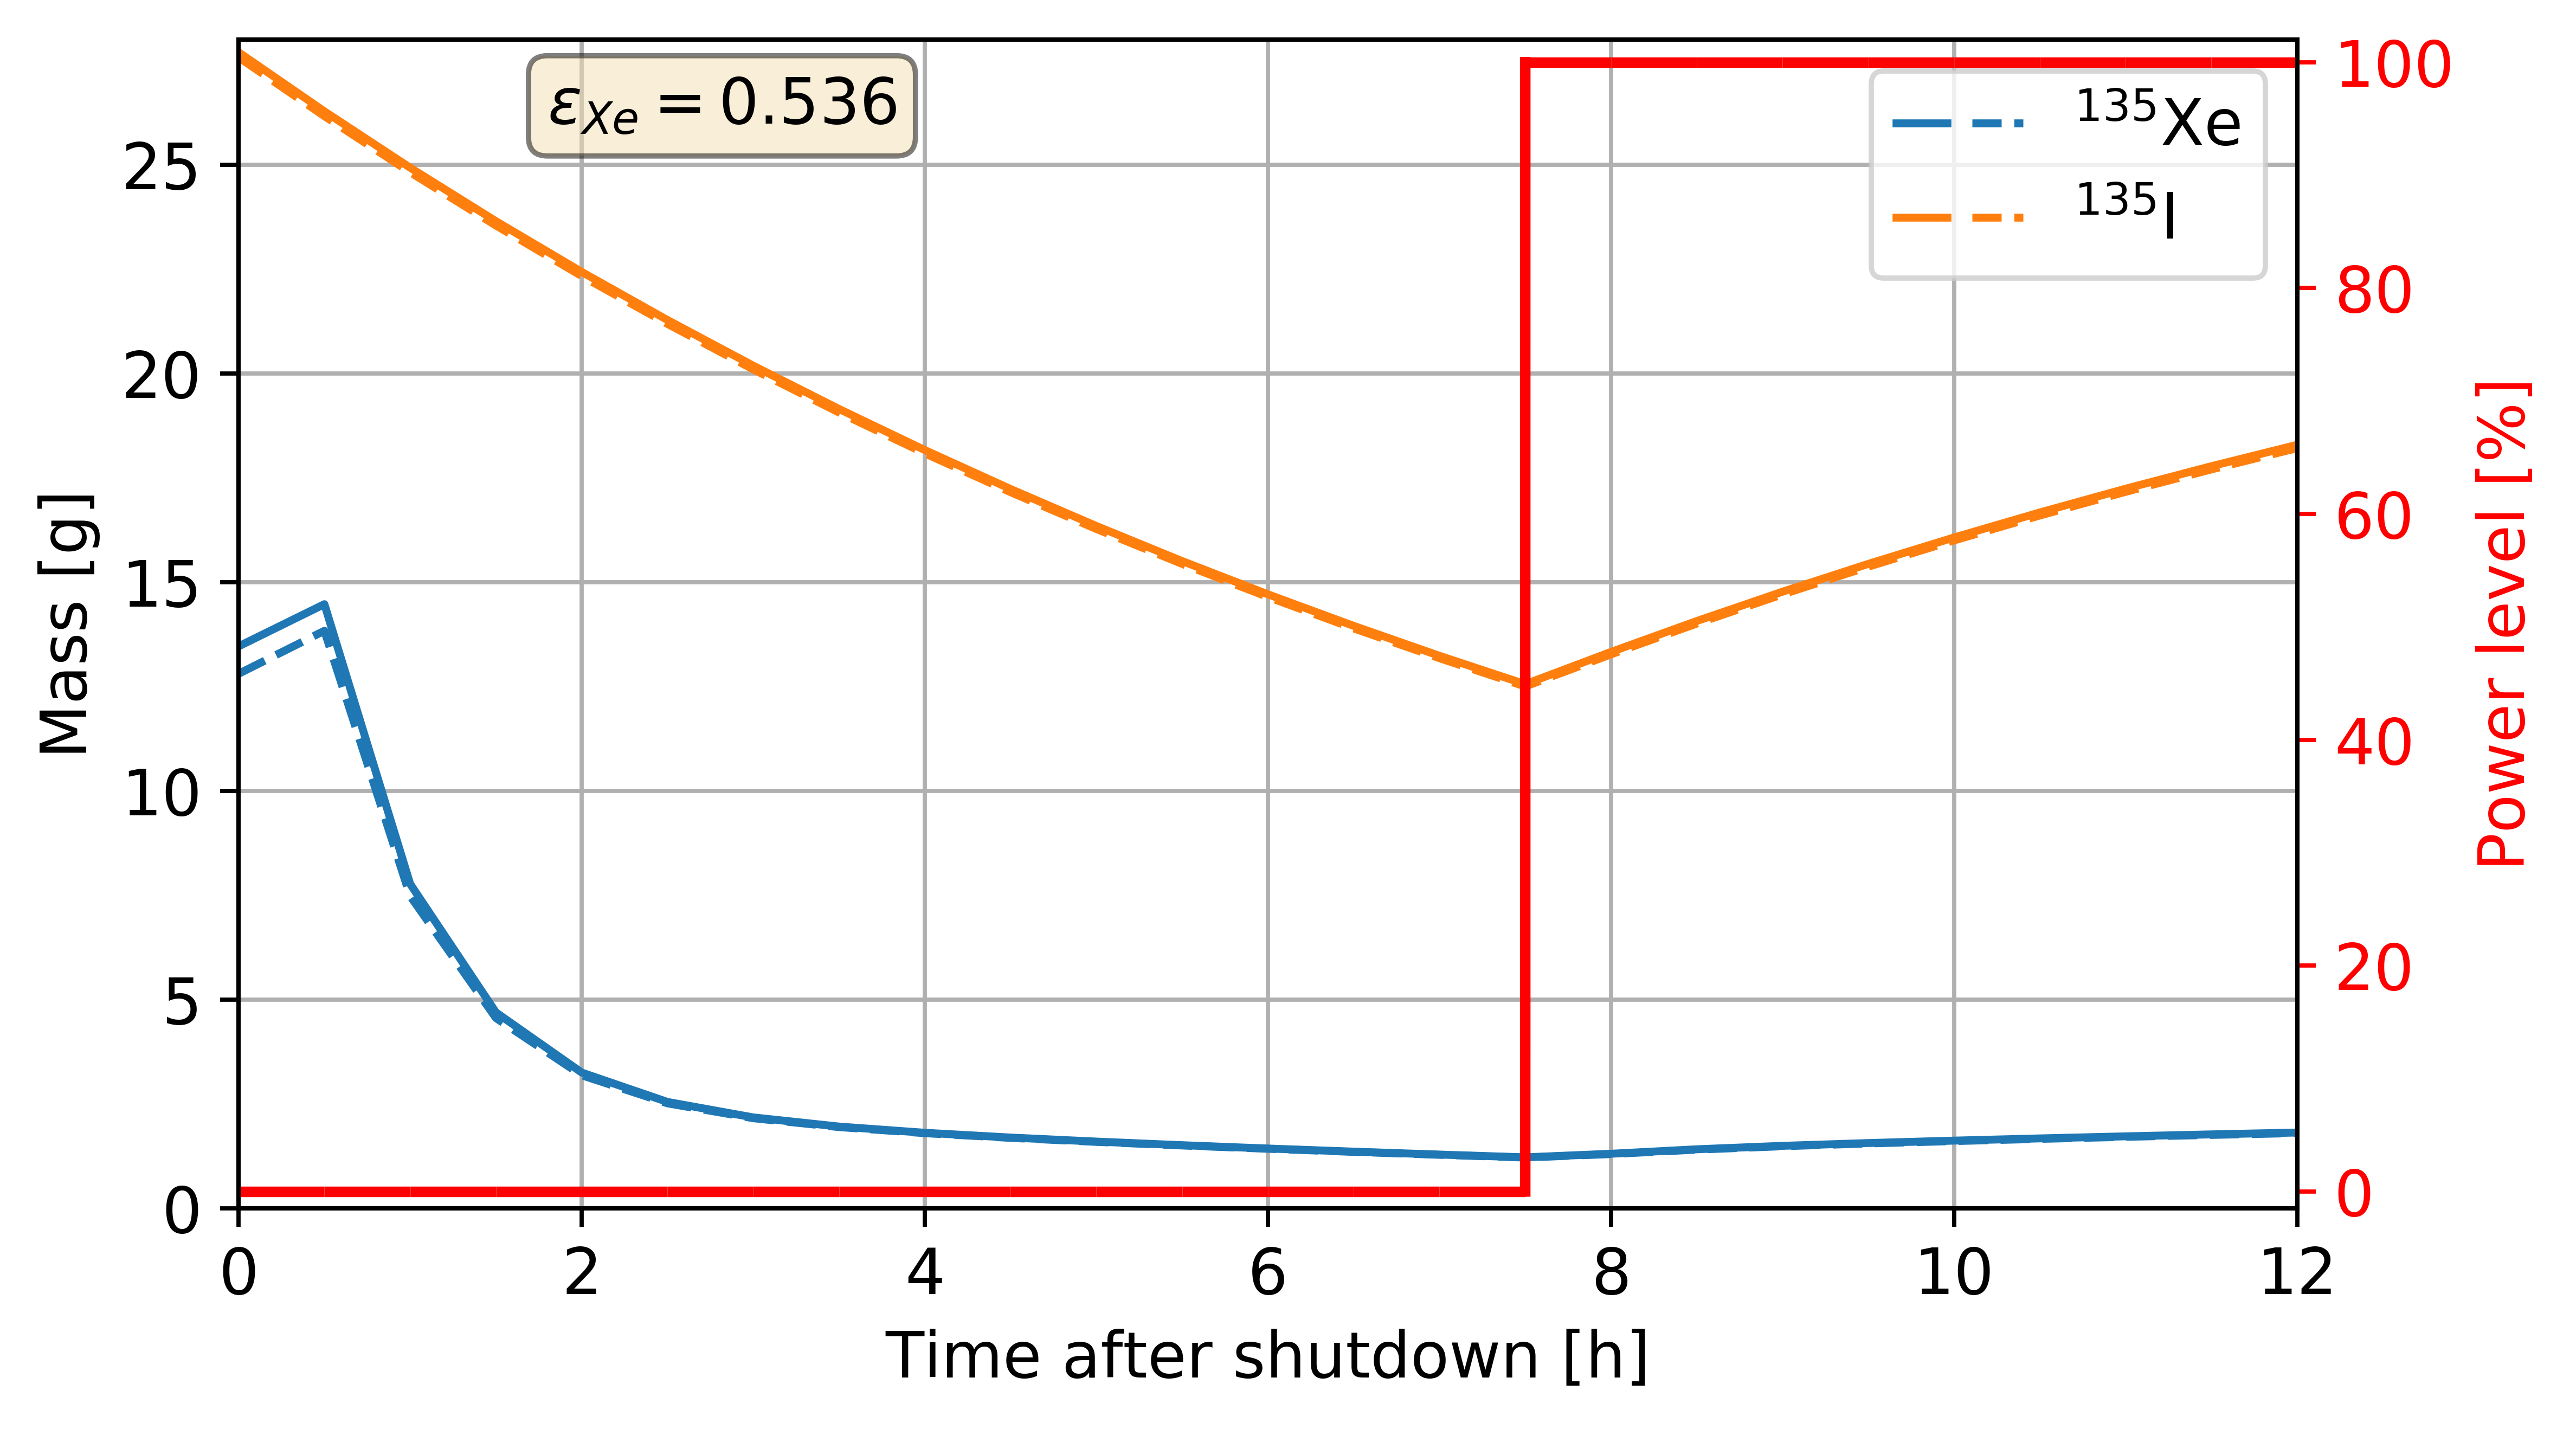
\includegraphics[width=0.88\textwidth]{ch6/kl25_xe_i_ratio.png}\vspace{-13mm}\\
	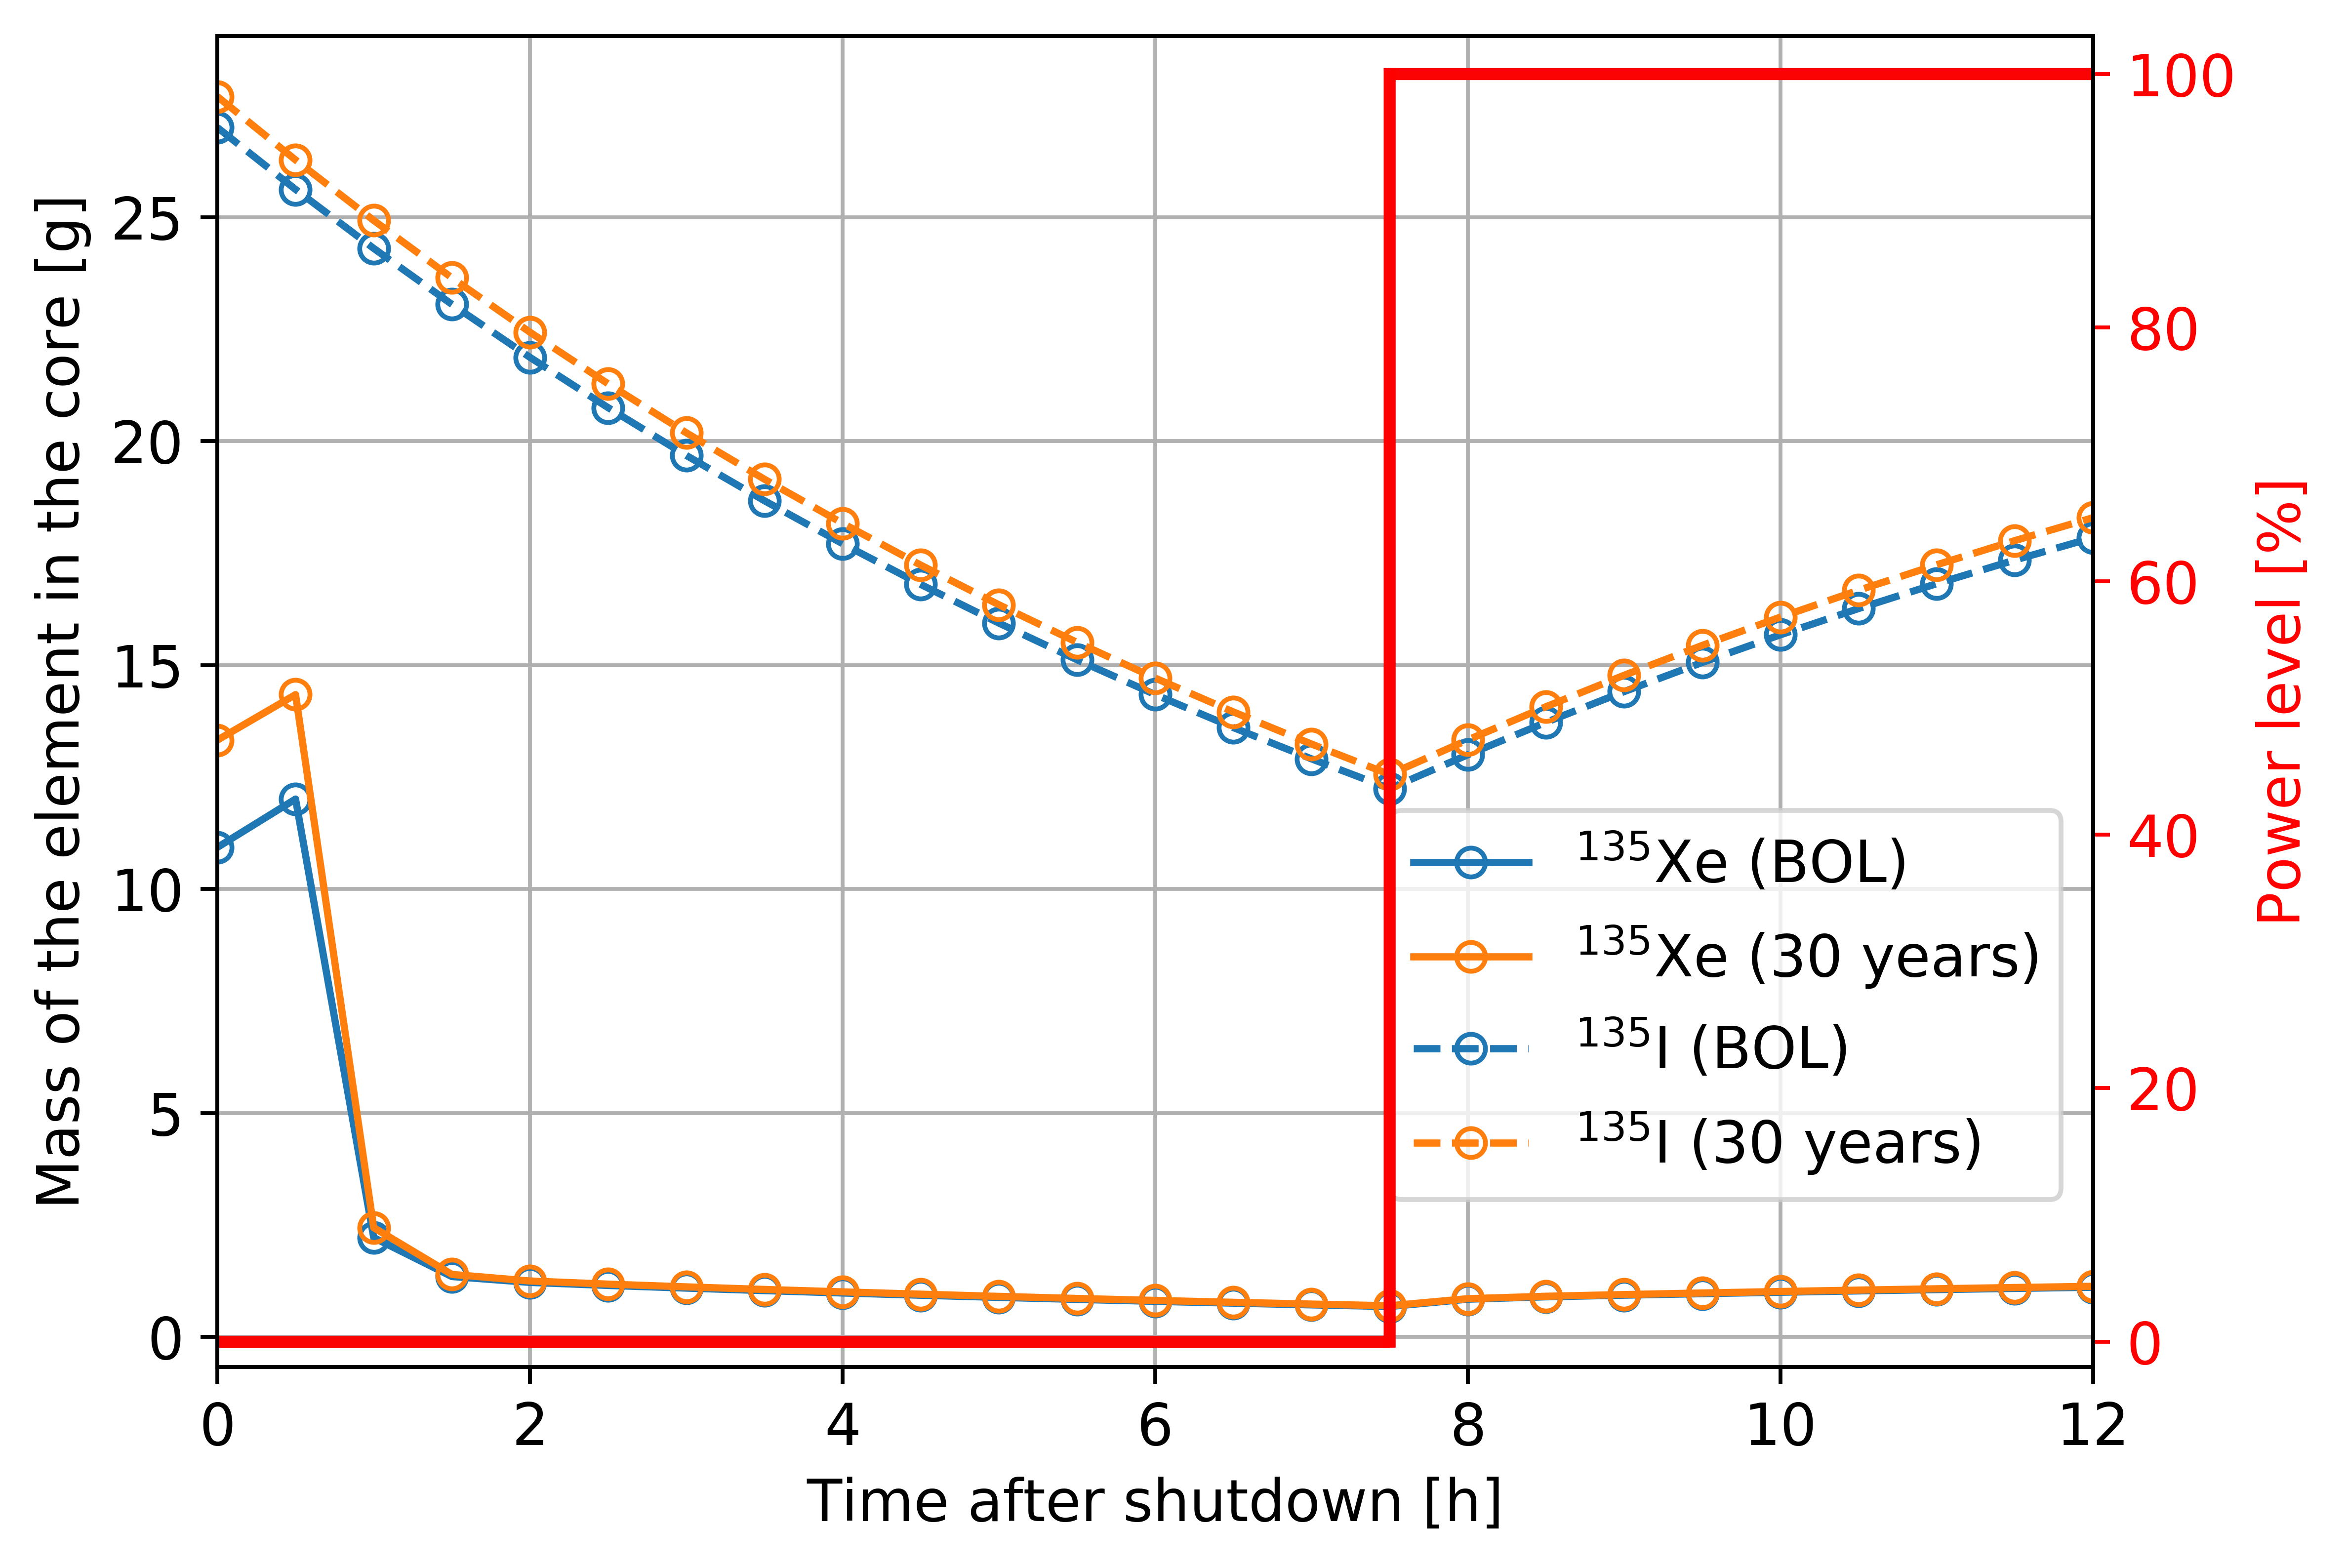
\includegraphics[width=0.88\textwidth]{ch6/kl100_xe_i_ratio.png}
	\end{array}$
	\vspace{-4mm}
	\caption{Comparison of $^{135}$Xe and $^{135}$I isotopic content at the 
		\gls{BOL} (dashed line) and after 30 years of operation (solid line) 
		for 
		various gas removal regimes. The uncertainty $\pm\sigma$ is shaded.}
	\label{fig:msbr-lf-xe-i-ratio}
\end{figure}

Such a large 
variations in $^{135}$Xe concentration are observed due to batch-wise nature 
of SaltProc simulations (e.g., the fraction of target poison is being 
removed discretely, at the end of each depletion step). Realistically, the gas 
removal system extracts gas from the fuel salt continuously, which would 
result in a much smoother change in the concentration and, accordingly, 
in the reactivity. Notably, for the both \gls{BOL} and \gls{EOL}, the 
$^{135}$Xe mass stabilized at 1 g in about 3-4 hours after the shutdown and 
started inclining slowly ($60$ $mg/EFPH$) after power ramp-up from 0 to 100\%. 
That is, when the reactor operates again on a full-power level,  $^{135}$Xe 
concentration during a few days will be significantly lower than before 
load-following transient. Thus, less thermal neutrons will be parasitically 
absorbed in the fission gas. As a result, the long-term fuel cycle performance 
metrics such as fuel utilization and the core lifetime would benefit 
enormously from a ``clean-up" effect of the postulated transient, but such 
analysis is out of scope of this work.

In the case of moderate gas removal efficiency, major fission product 
concentration changes very similar to high removal efficiency case. The 
$^{135}$I/$^{135}$Xe concentration ratio is 2.15 and 2.06 at the \gls{BOL} and 
after 30 years of full-power operation, respectively, and caused 7.5\% hike 
in $^{135}$Xe concentration. Surprisingly, significantly lower gas removal 
efficiency ($\epsilon_{Xe}=0.536$ instead of 0.915) provided comparable 
benefits to the core neutronics during the postulated load-following 
transient. In fact, similarly to the $\epsilon_{Xe}=0.915$ case, the 
$^{135}$Xe mass stabilized at 1.5 g in about 5 hours after the shutdown and 
then increasing slowly ($165$ $mg/EFPH$) after power ramp-up from 0 to 100\%.
In conclusion, simpler and cheaper gas removal system with extraction 
efficiency $\epsilon_{Xe}=0.536$ enough to suppress the xenon poisoning effect 
after shutdown to acceptable level (-161 $pcm$) and to ensure load-following 
capability of the \gls{MSBR}.


\subsection{Neutron spectrum}
Figure~\ref{fig:ch6-msbr-spectrum} shows that the \gls{MSBR} spectrum after 30 
years of operation (solid line) is harder than at the startup (dashed line). 
Compared to the \gls{MSBR}, the \gls{TAP} \gls{MSR} spectrum is significantly 
harder even when all moderator rods are inserted to the core. Notably, the 
\gls{MSBR} spectrum has clear peak in thermal energy region, but flat neutron 
energy dependence in intermediate and fast energy region, which is quite 
common for thermal reactors. In contrast, the \gls{TAP} core spectrum at the 
\gls{EOL} has high peak in fast and lower peak in thermal energy region, 
which is typical for epithermal/intermediate reactors. This is main reason, 
why for the postulated load-following transient I observed significant xenon 
poisoning effect in the \gls{MSBR} and negligible xenon impact in the 
\gls{TAP} \gls{MSR} (see Chapter 5).
\begin{figure}[htbp!] % replace 't' with 'b' to 
	\centering
	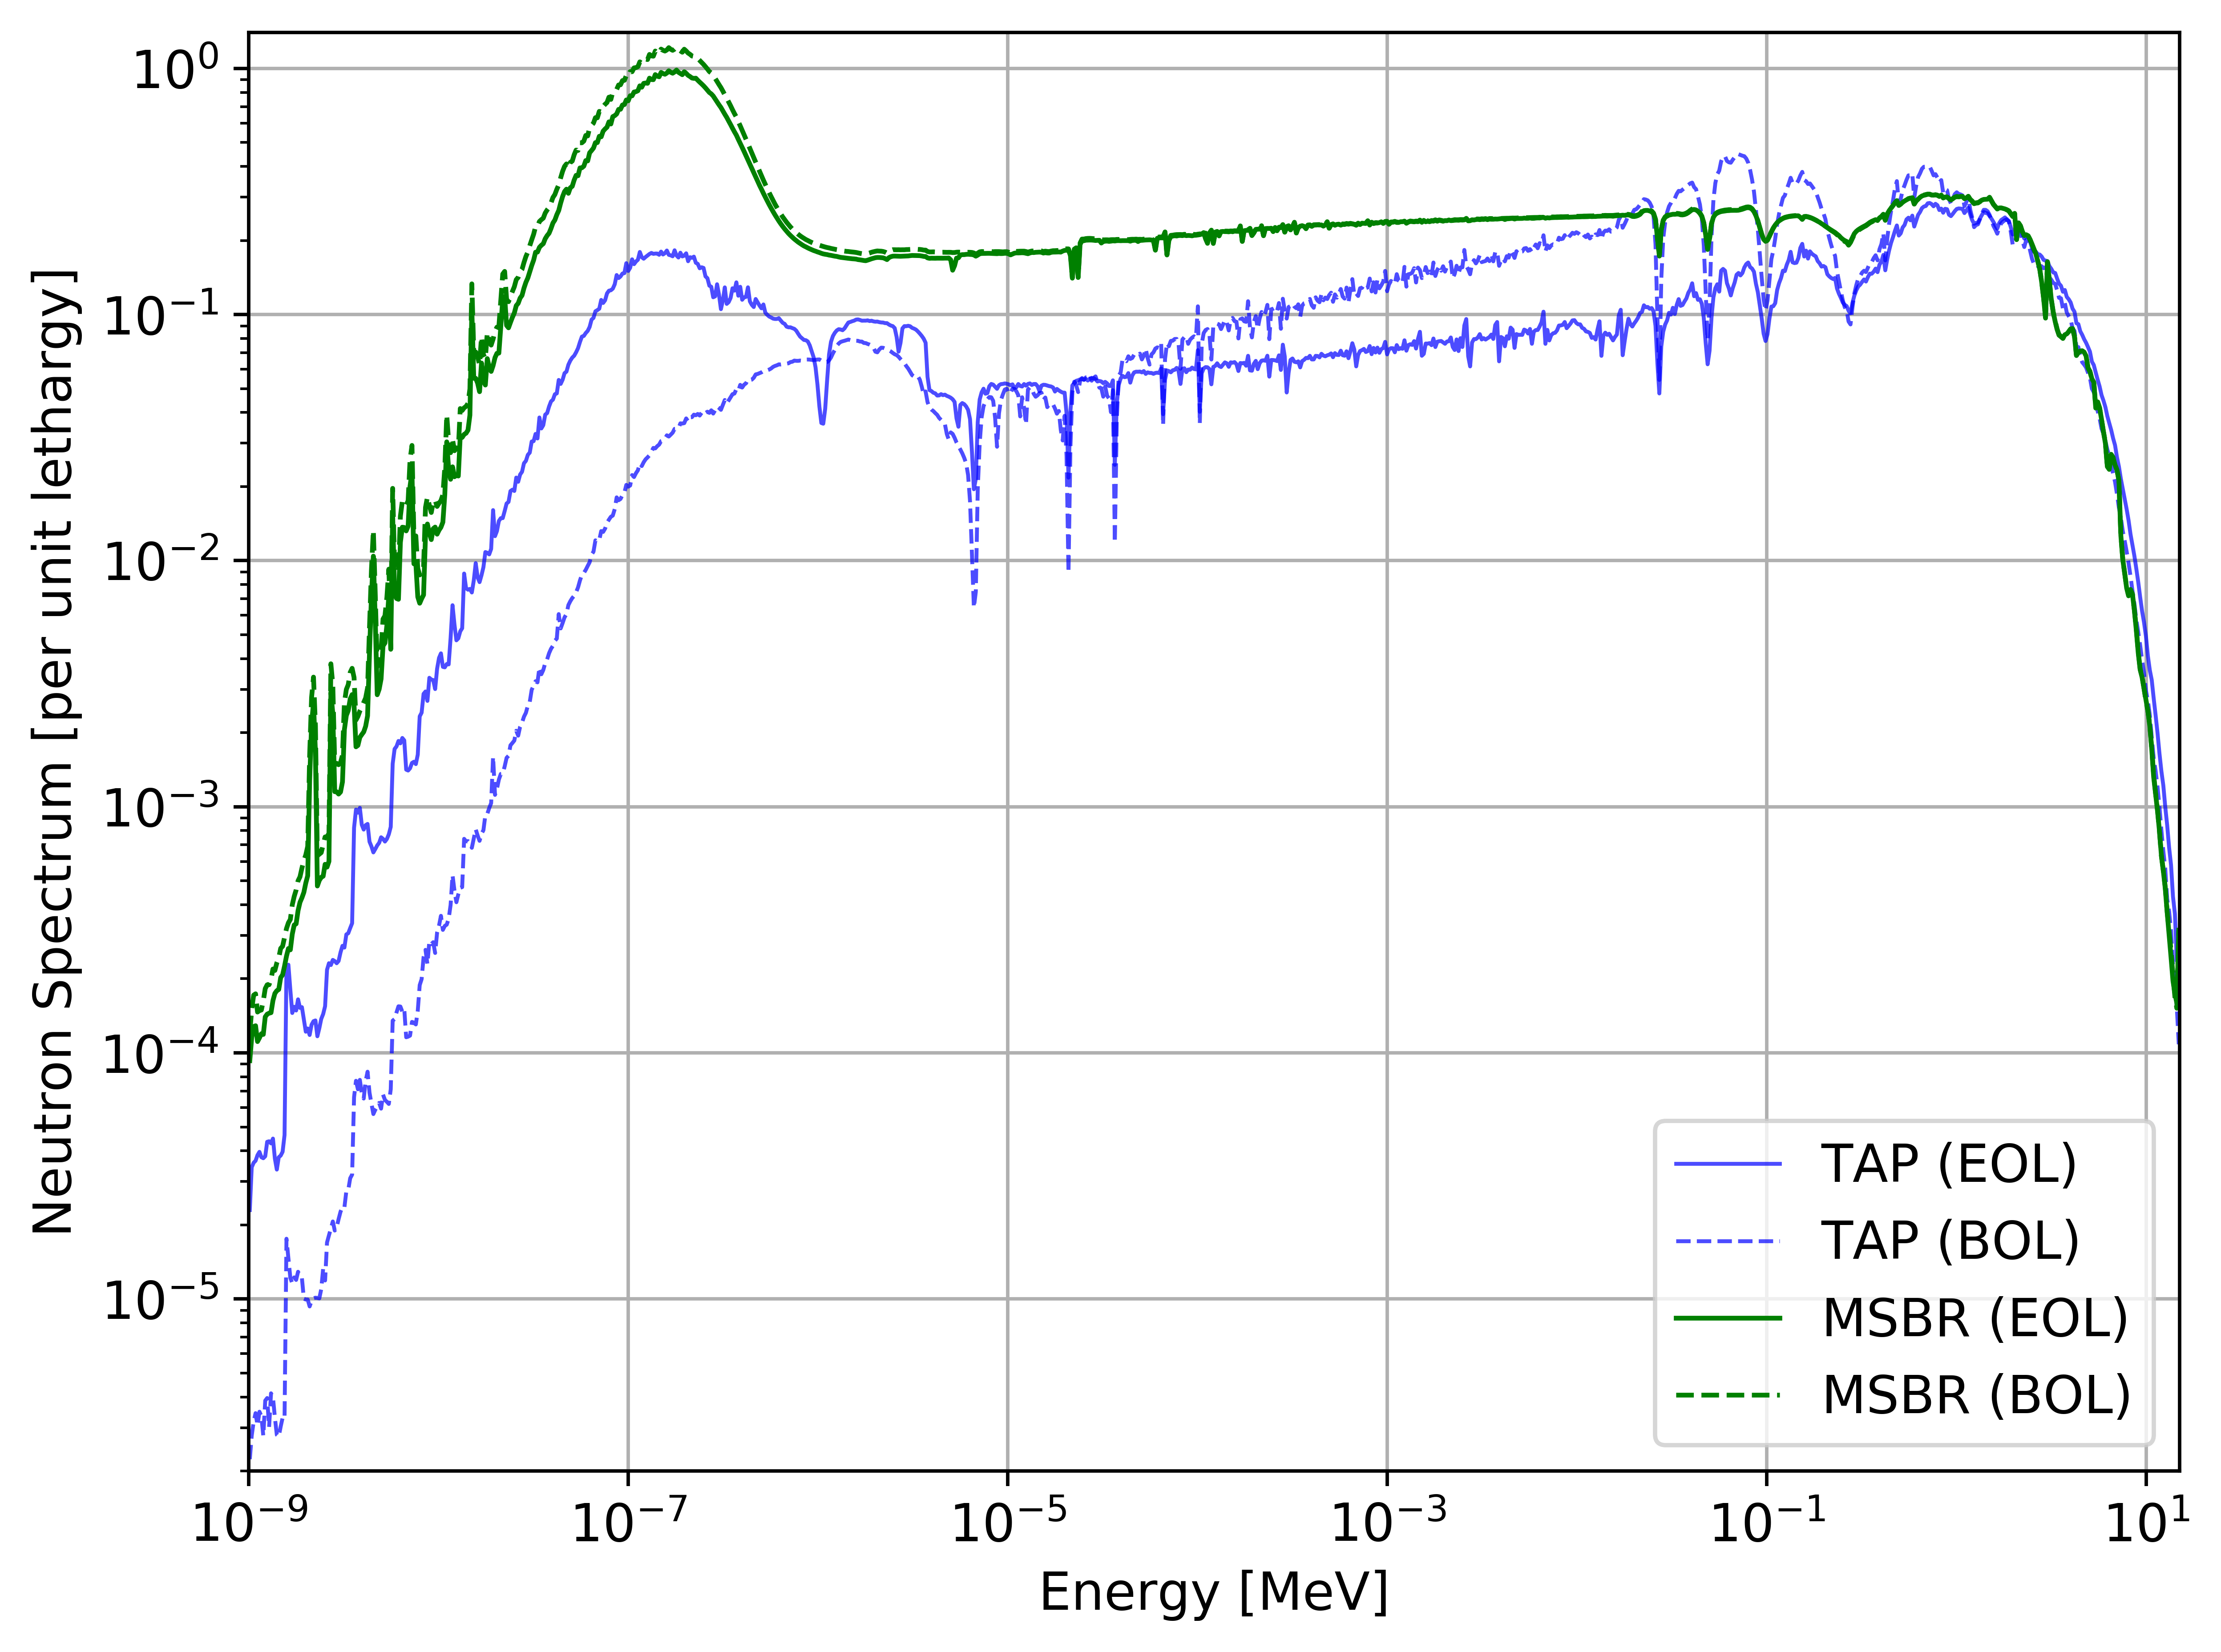
\includegraphics[width=\textwidth]{ch6/msbr_vs_tap_spectrum.png}
	\caption{Neutron spectra normalized by lethargy for the \gls{MSBR} and 
		\gls{TAP} at various moments during operation. The neutron flux 
		uncertainties $\sigma_{\Phi}$ are 0.6\% and 0.18\% for the \gls{TAP} 
		reactor and \gls{MSBR}, respectively.}
	\label{fig:ch6-msbr-spectrum}
\end{figure}

Potentially, any graphite-moderated liquid-fueled \gls{MSR} conceptual 
design\footnote{Integral Molten Salt Reactor (IMSR) from Terrestial Energy 
\cite{leblanc_integral_nodate}, Molten Salt Demonstration Reactor (MSDR) from 
Oak Ridge National Laboratory \cite{bettis_design_1972}, Liquid fluoride 
thorium reactor (LFTR) from Flibe energy \cite{sorensen_liquid-fluoride_2016}, 
etc.} would demonstrate similar benefits from the presents of the online gas 
removal system within nuclear island.


\section{Safety and operational parameters}
The significant changes of strong absorbers concentration in the fuel slightly 
shift the core spectrum which potentially might impact the reactor safety.
Rapid changes in fuel salt composition should not compromise critical safety 
margins.
I calculated major safety and operational parameters at various moments 
throughout the postulated transient using approaches from 
Sections~\ref{sec:safety-param} and \ref{ch5:saf_param}. 
The total temperature coefficient of reactivity ($\alpha_{ISO}$) must remain 
negative and the total control rod worth (CRW) must be sufficient to trip the 
reactor throughout the postulated transient. Ideally, we want to major safety 
and operational parameters stay almost constant because the changes in those 
parameter would require fast response from reactor control systems (i.e., the 
control rod jerk in response to the CRW change).

\subsection{Temperature coefficient of reactivity}
Figure~\ref{fig:msbr-lf-tc-evo} shows the temperature feedback coefficient 
dynamics for the \gls{MSBR} during the transient for various gas removal 
efficiencies ($\epsilon_{Xe}=0.536$ and 0.915). 
The Fuel Temperature Coefficient ($\alpha_{T,F}$) becomes less negative at the 
beginning of the transient for all cases. The reason for this is a 
slight spectrum hardening due to the $^{135}$Xe concentration peak changed the 
Doppler broadening of resonances. After that, the magnitude of $\alpha_{T,F}$ 
slowly inclined due to $^{135}$Xe removal from the fuel.
\begin{figure}[htbp!] % replace 't' with 'b' to 
	\centering
	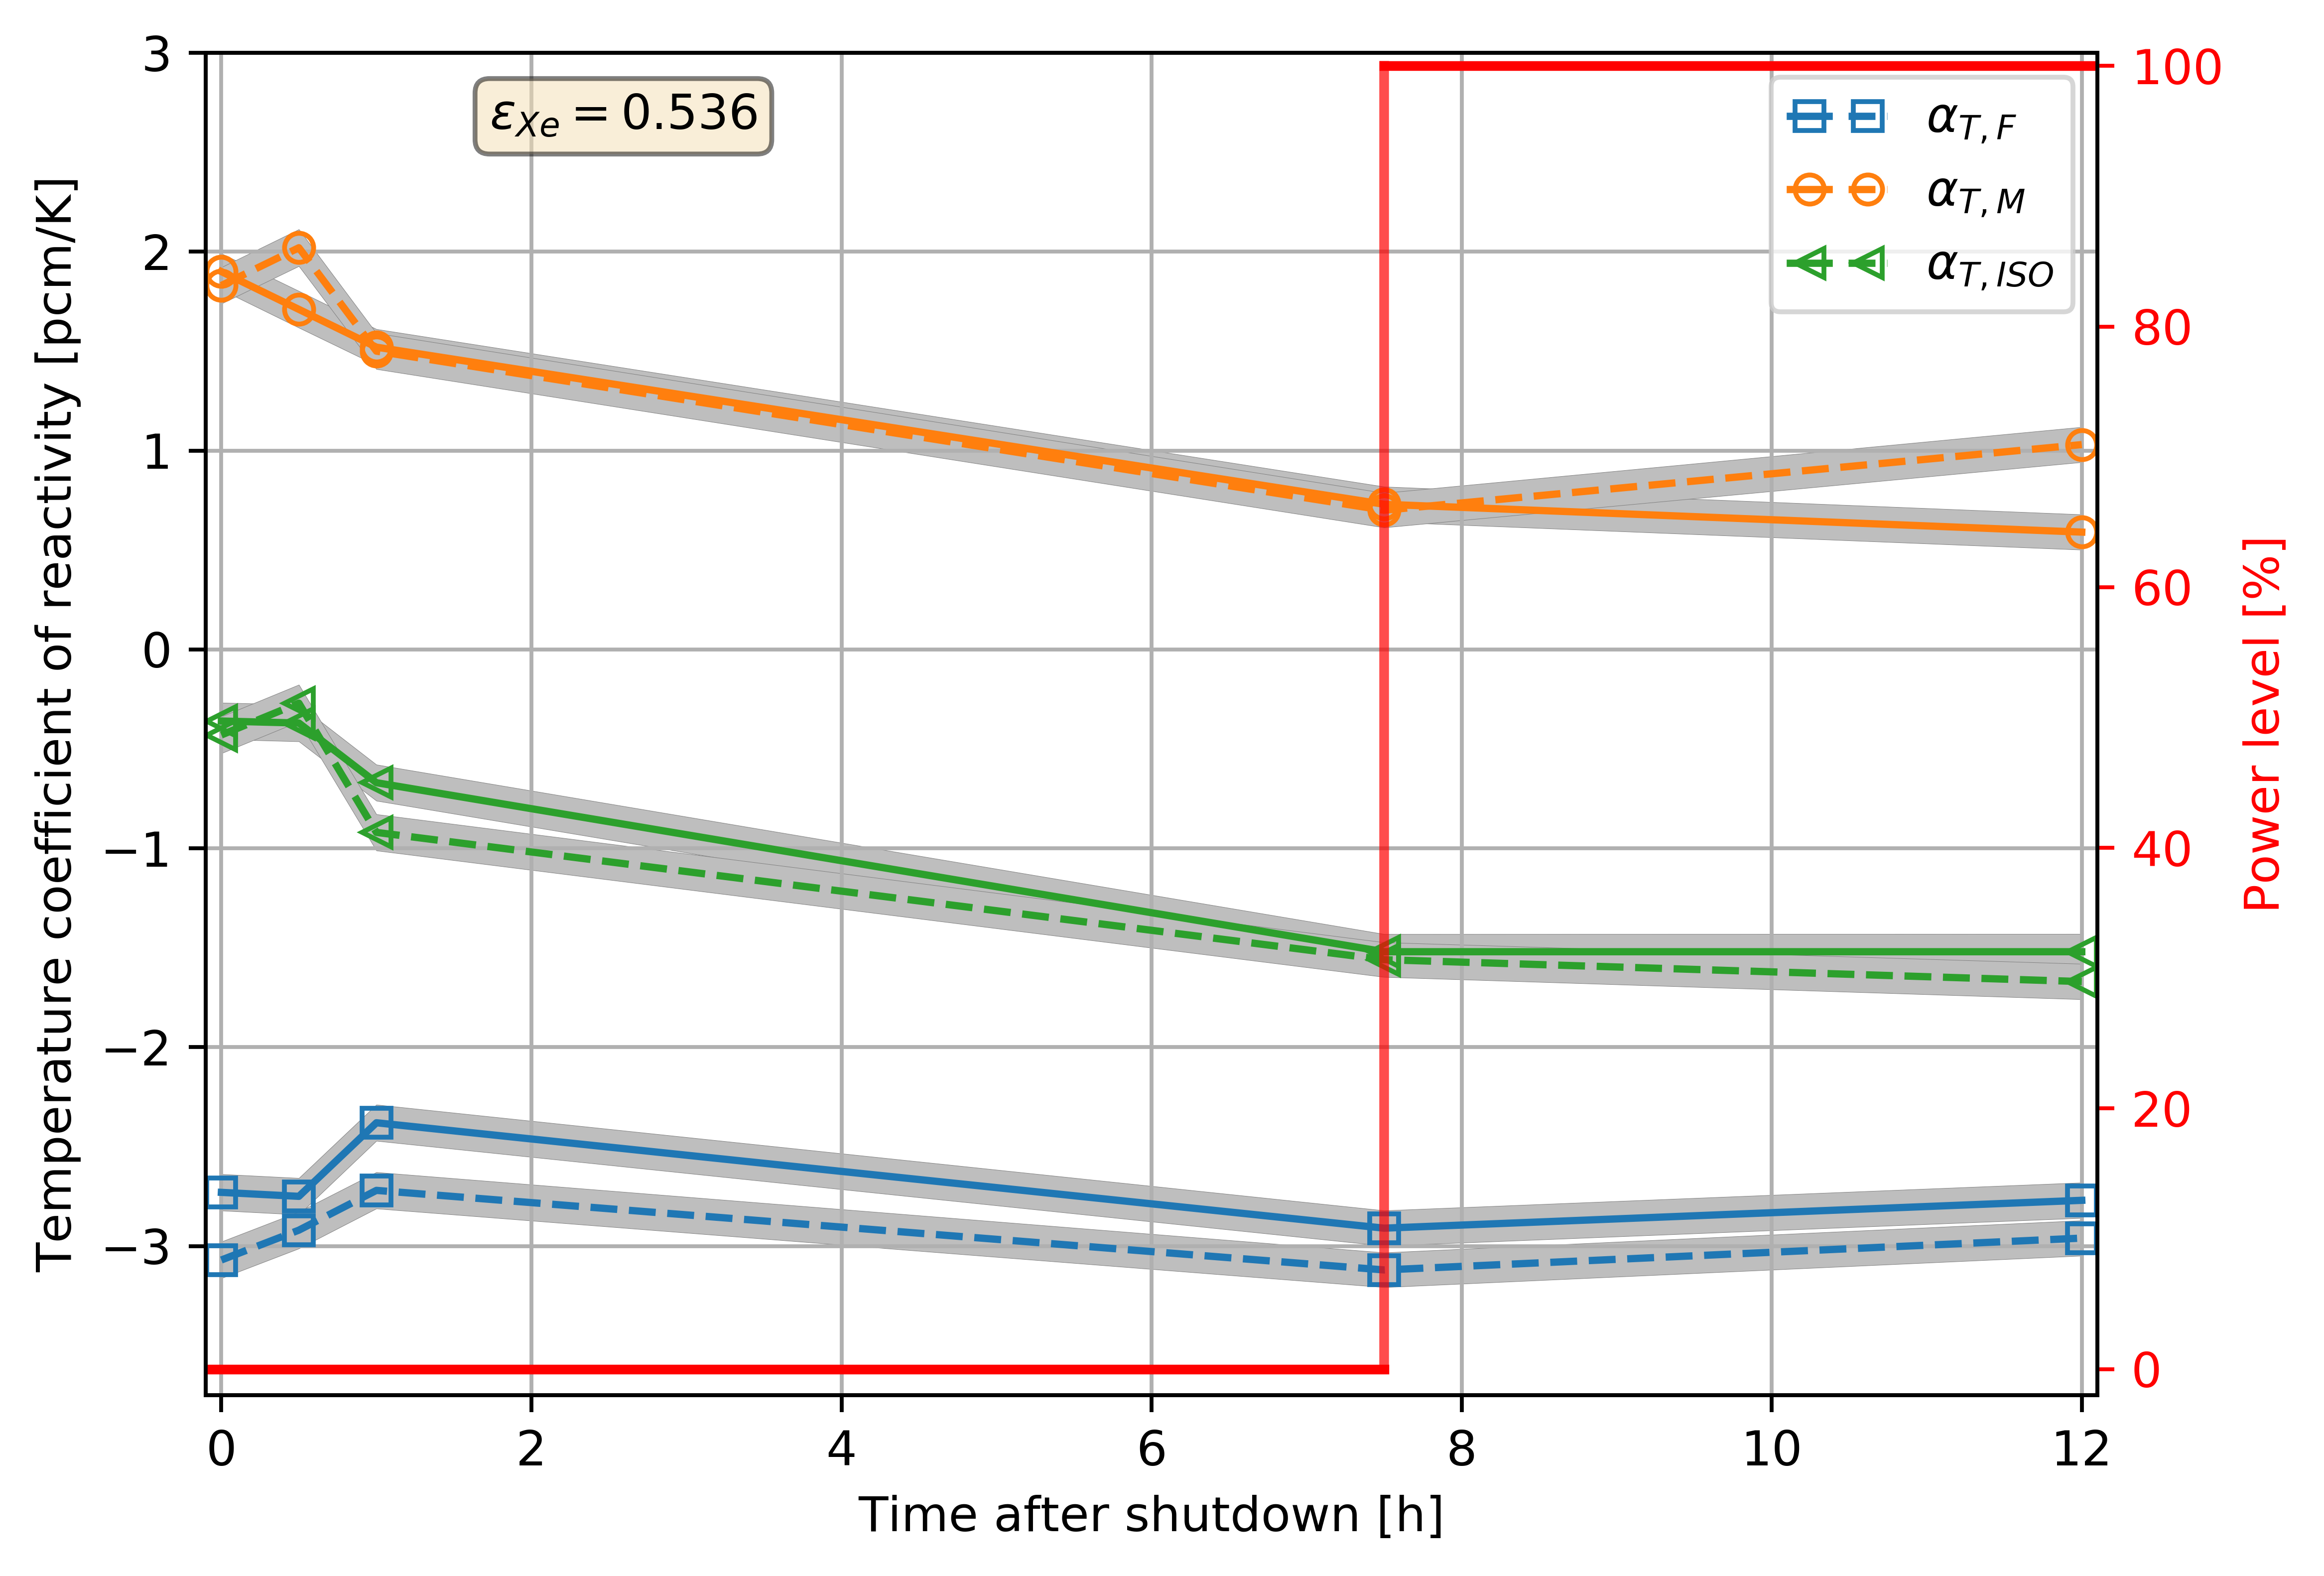
\includegraphics[width=0.95\textwidth]{ch6/saf_par/tc_evo_kl25.png}\\
	\vspace{-12mm}
	\hspace{+0.05mm}
	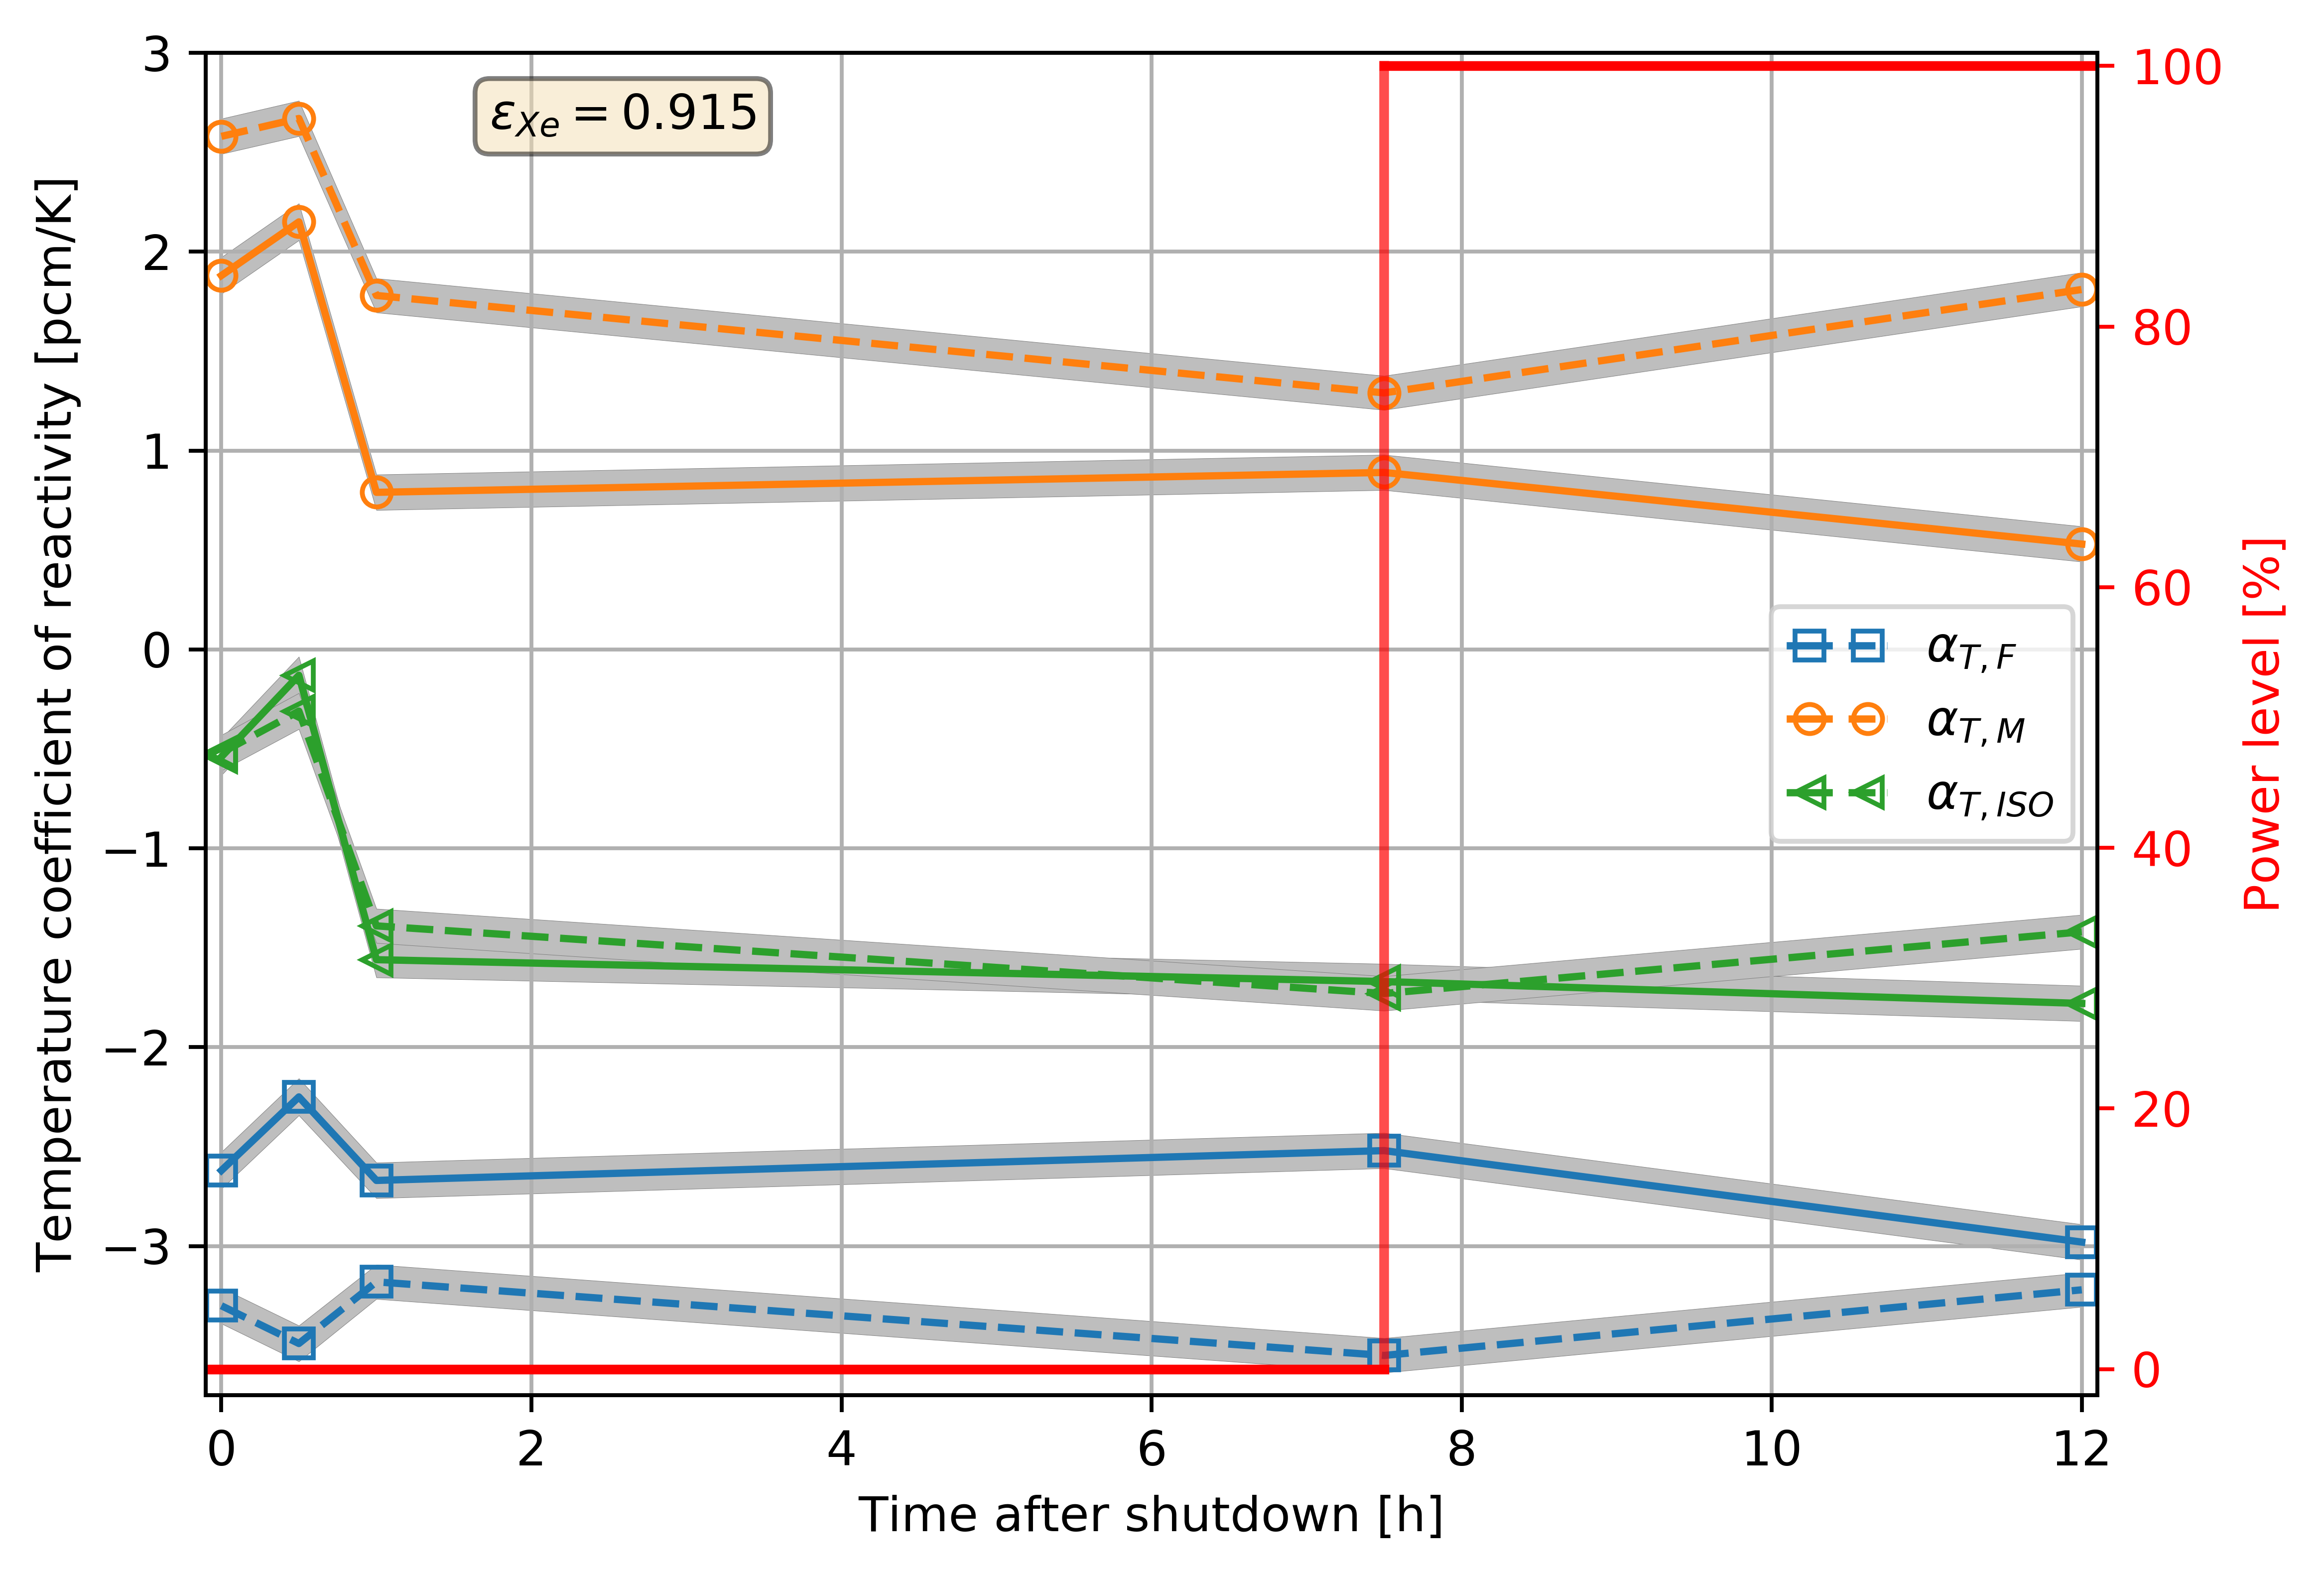
\includegraphics[width=0.95\textwidth]{ch6/saf_par/tc_evo_kl100.png}
	\vspace{-3mm}
	\caption{Temperature feedback coefficients during the postulated transient 
	for the \gls{MSBR} operating with moderate ($\epsilon_{Xe}=0.536$, upper) 
	and high ($\epsilon_{Xe}=0.915$, lower) gas removal efficiency at the 
	\gls{BOL} (dashed line) and after 30 years of operation (solid line).
	The	uncertainty $\pm\sigma$ is shaded.}
	\label{fig:msbr-lf-tc-evo}
\end{figure}

The isothermal temperature coefficient, $\alpha_{ISO}$, is $-0.36\pm0.09$ 
$pcm/K$ at the beginning and remains stable during first 30 minutes of the 
transient for the moderate removal efficiency case.  Then, as the gas removal 
system reduces $^{135}$Xe concentration in the core, $\alpha_{ISO}$ becomes 
even more negative: $-1.52\pm0.09$ $pcm/K$ when the $^{135}$Xe mass stabilized 
at 1.5 g in about 5 hours after the shutdown. After power ramp-up from 0\% to 
100\%, $\alpha_{ISO}$ remains stable since the $^{135}$Xe mass increasing very 
slowly. On the whole, another interesting benefit from the online gas removal 
is improved passive safety (stronger temperature feedback coefficient) 
throughout and, possibly, a few days after the postulated transient due to low 
concentration of the $^{135}$Xe in the fuel salt.

For the high gas removal efficiency regime ($\epsilon_{Xe}=0.915$), the 
isothermal temperature coefficient worsens from $-0.54\pm0.09$ $pcm/K$ to 
approximately $-0.22\pm0.09$ $pcm/K$ during first 30 minutes after shutdown. 
Afterwards, when the gas removal system extracted major fraction of the 
$^{135}$Xe from the fuel salt, $\alpha_{ISO}$ became significantly more 
negative ($-1.39$ and $-1.56$ $pcm/K$ at the \gls{BOL} and after 30 years of 
operation, respectively) due to the spectrum softening.

Overall, the combination of fuel and moderator thermal feedback coefficients, 
$\alpha_{ISO}$, remains negative throughout the postulated transient. 
Moreover, simpler and cheaper gas removal system with extraction 
efficiency $\epsilon_{Xe}=0.536$ provided more predictable thermal feedback 
coefficient dynamics throughout the transient due to 
a more gradual change in the $^{135}$Xe concentration.

\subsection{Void coefficient of reactivity}
Figure~\ref{fig:msbr-tap-void-evo} demonstrates the void coefficient of 
reactivity evolution during the postulated transient. 
The $\alpha_V$ remains almost constant throughout the transient for all cases. 
Notably, the void coefficient of reactivity after 30 years of full-power 
operation is substantially greater than at the startup for both gas removal 
regimes. Thus, the unexpected void insertion due to the gas separation system 
failure would lead to more severe consequences toward \gls{EOL}. This 
observation should be taken into account in the \gls{MSBR} accident analysis 
and safety
justification.
\begin{figure}[htbp!] % replace 't' with 'b' to 
	\centering
	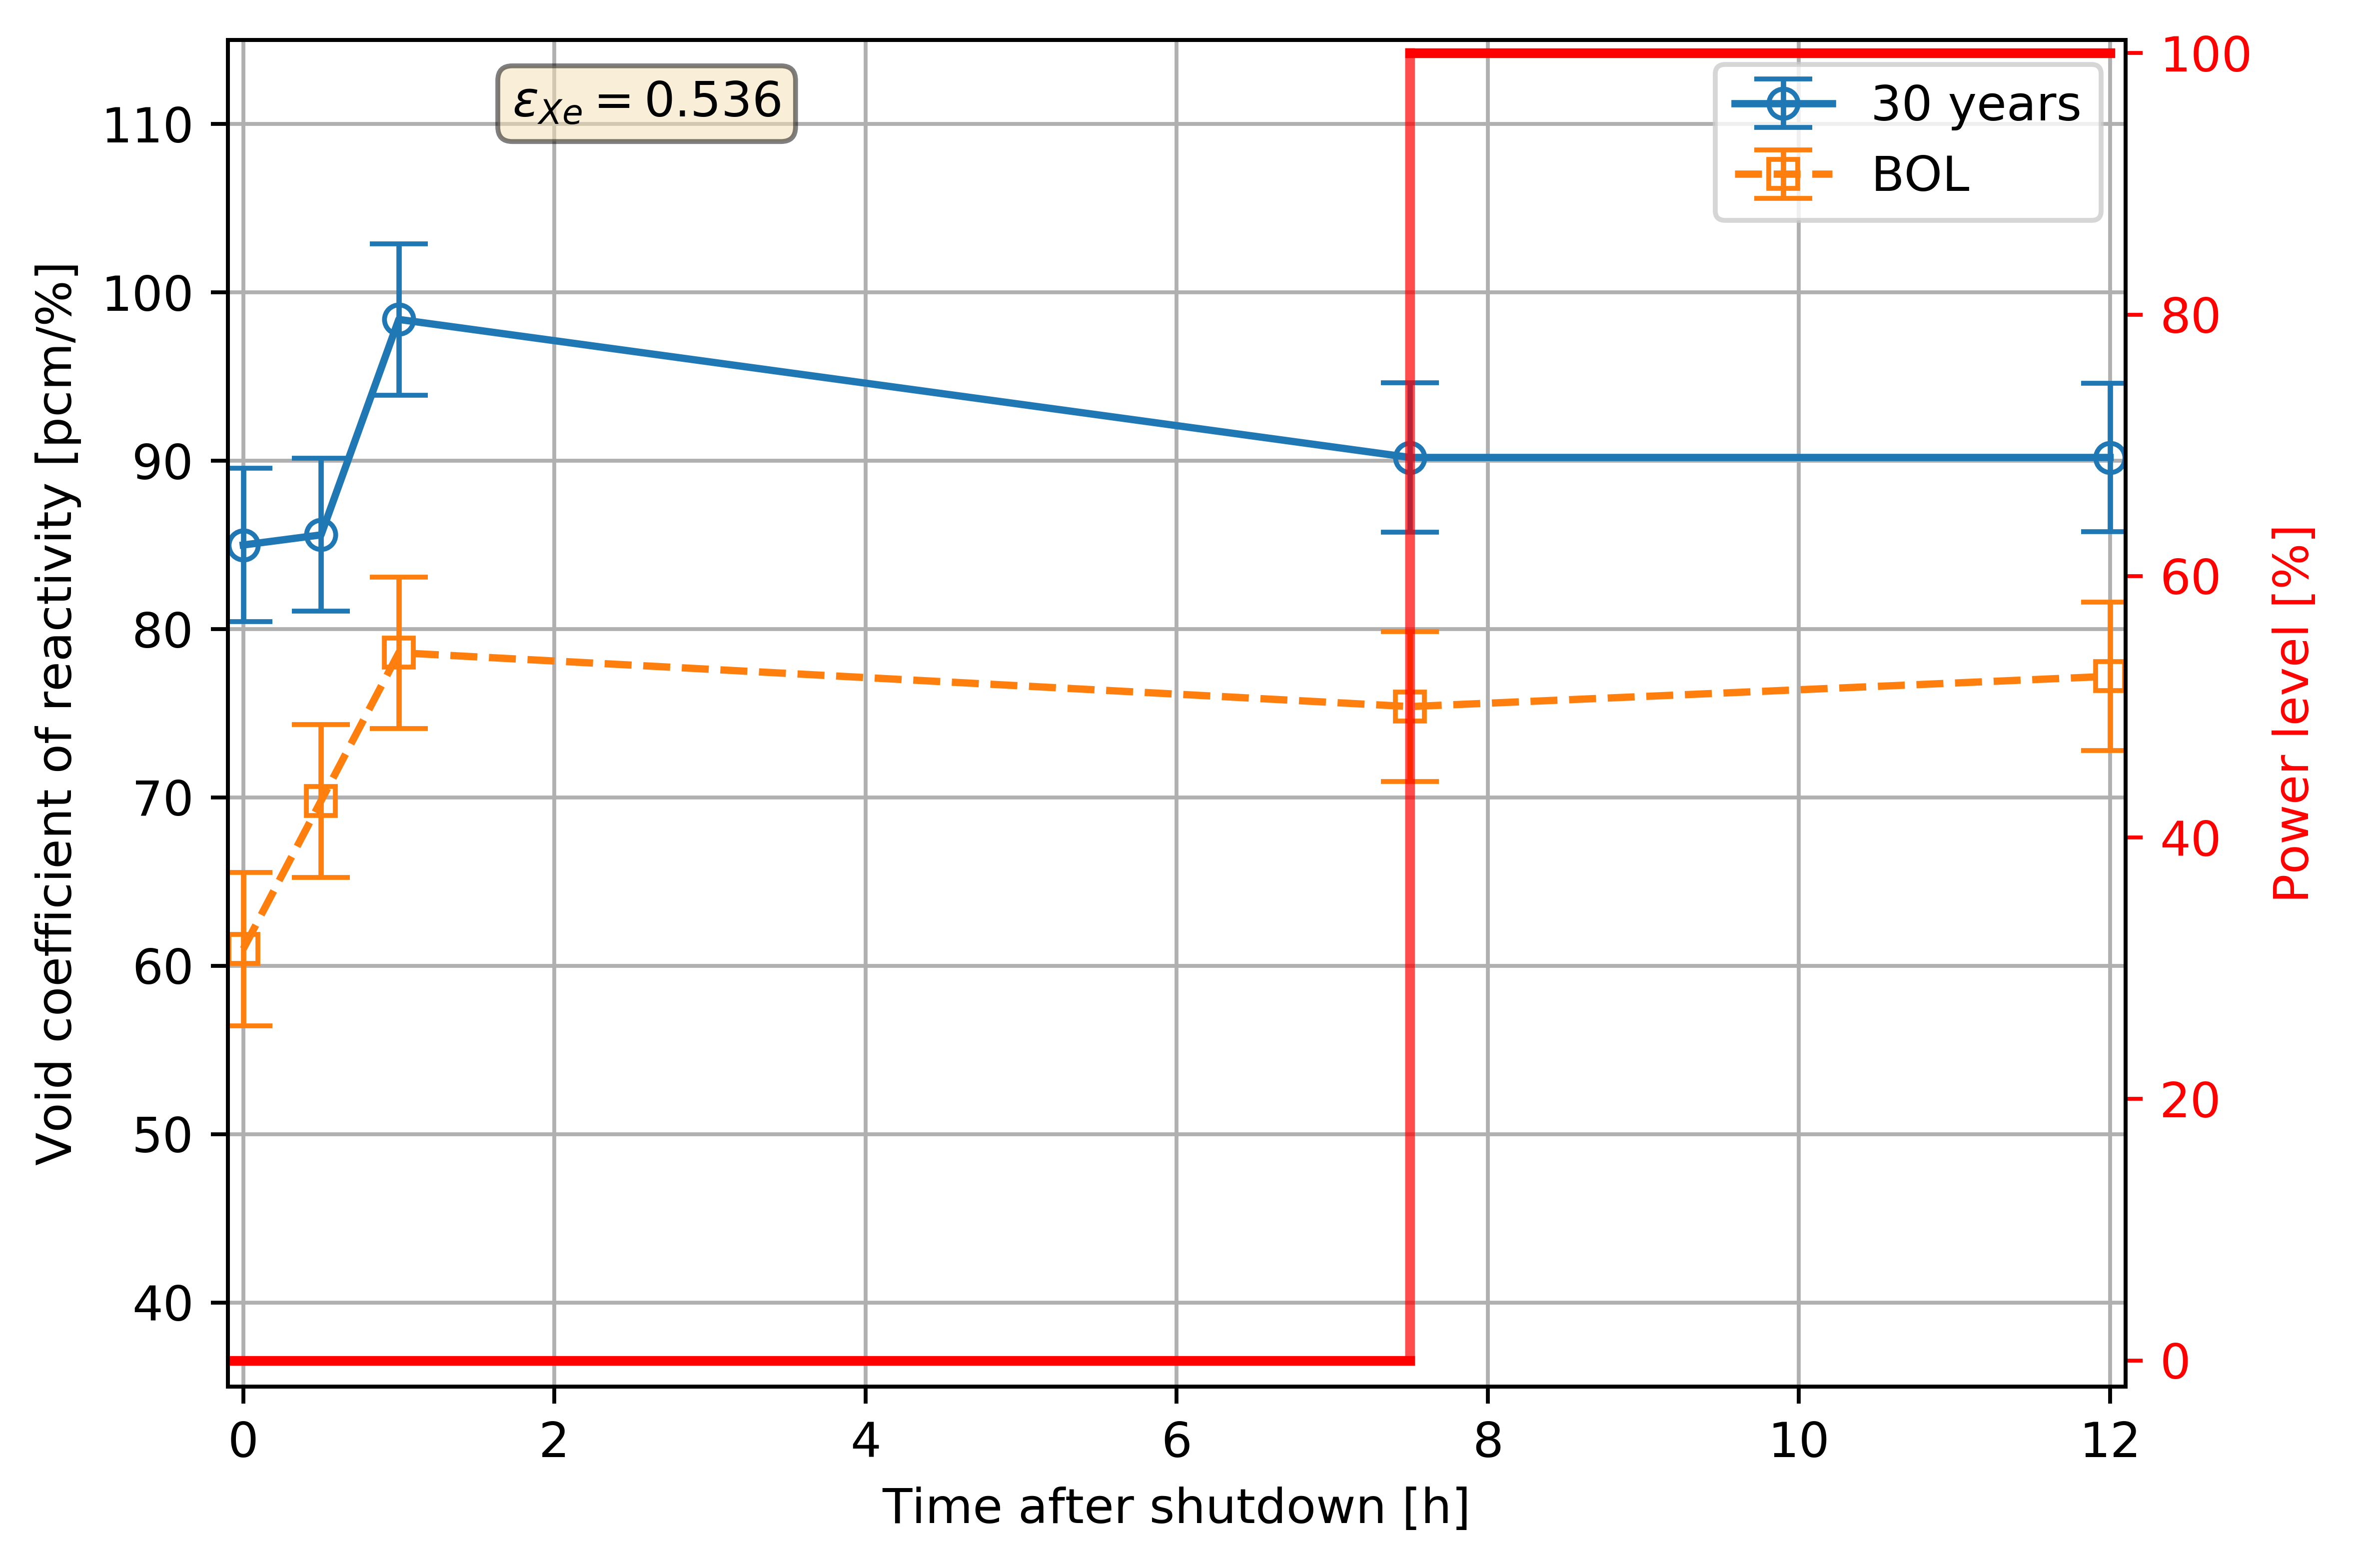
\includegraphics[width=0.95\textwidth]{ch6/saf_par/void_evo_kl25.png}\\
	\vspace{-12mm}
	\hspace{+0.05mm}
	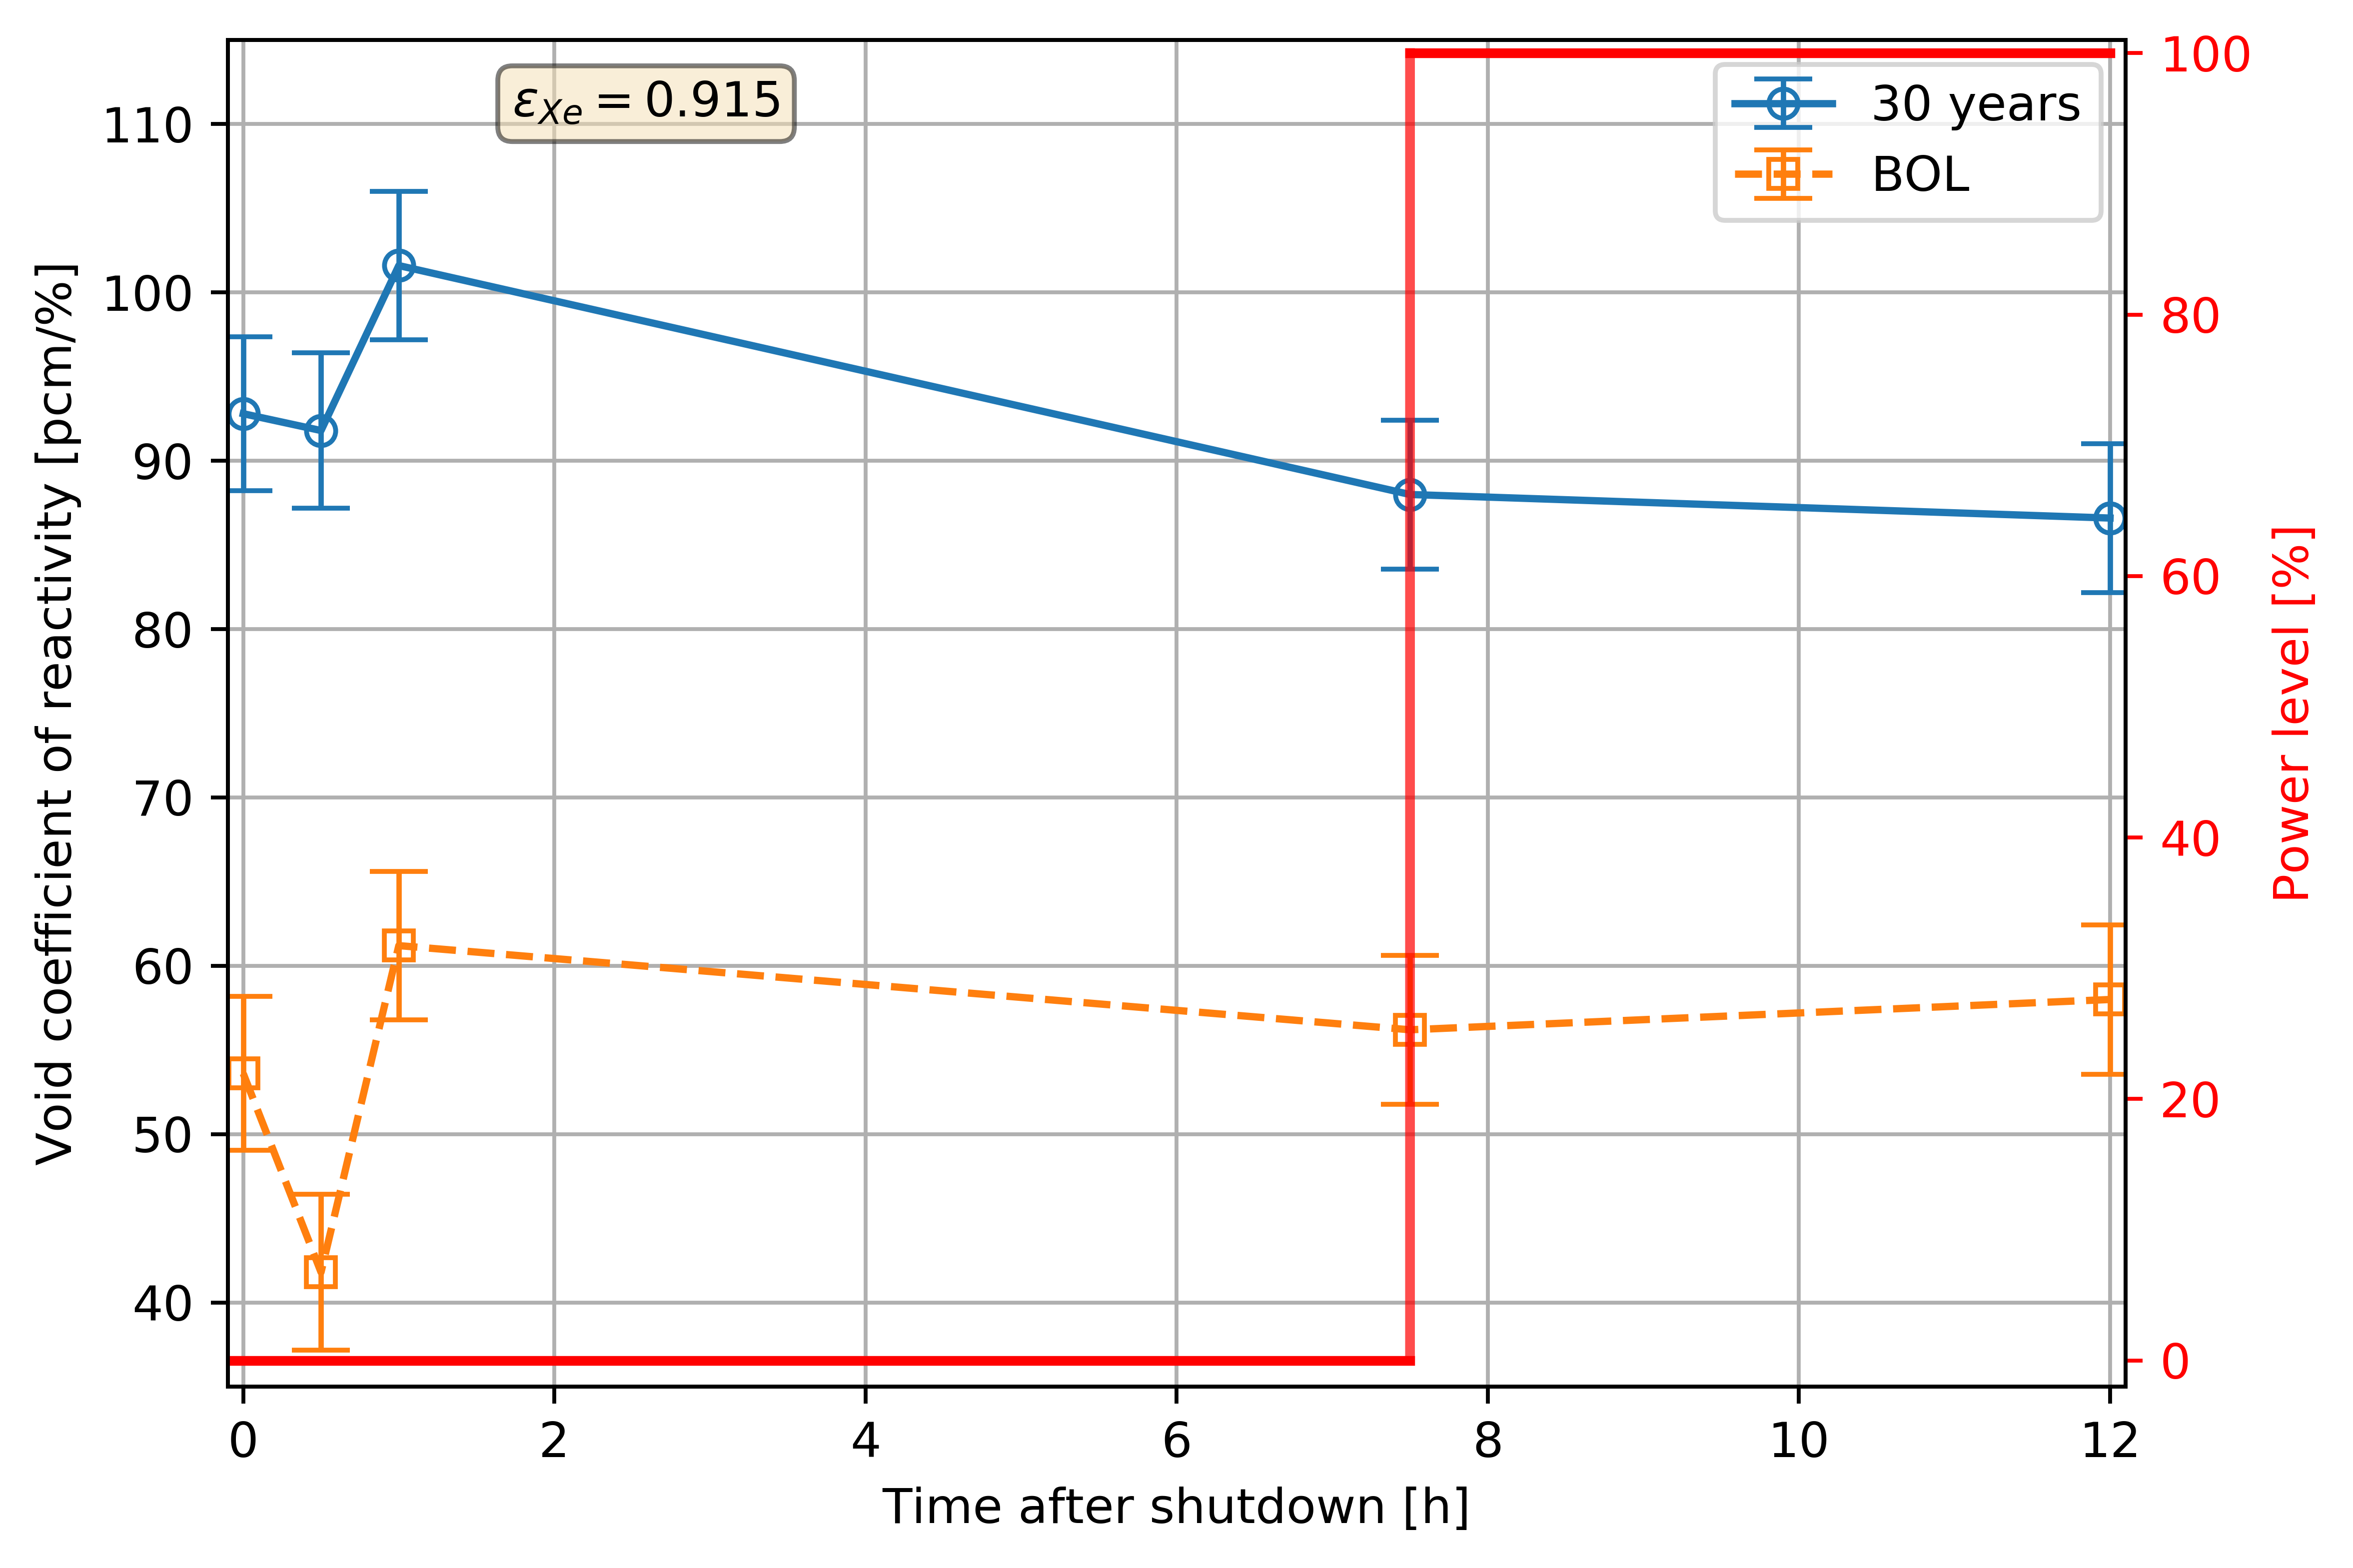
\includegraphics[width=0.95\textwidth]{ch6/saf_par/void_evo_kl100.png}
	\vspace{-3mm}
	\caption{Void coefficient of reactivity as a function of time during 
	postulated transient
for the \gls{MSBR} operating with moderate 
	($\epsilon_{Xe}=0.536$, upper) and high ($\epsilon_{Xe}=0.915$, lower) gas 
	removal efficiency at the \gls{BOL} (dashed line) and after 30 years of 
	operation (solid line). The uncertainty $\pm\sigma$ is shaded.}
	\label{fig:msbr-lf-void-evo}
\end{figure}

For the high gas removal efficiency case, $\alpha_V$ fluctuates during the 
postulated transient between 42 and 61 $pcm/$\% at the \gls{BOL} and between 
87 and 102 $pcm/$\% after 30 years of operation. The $^{135}$Xe concentration 
spike caused corresponding $\alpha_V$ drop due to short-term spectrum 
hardening. Then, $\alpha_V$ quickly recovers to its initial value. As for 
temperature feedback coefficient, the moderate gas removal efficiency provided 
more predictable $\alpha_V$ dynamics throughout the transient and smaller 
difference between $\alpha_V$ at the \gls{BOL} and \gls{EOL}.

\subsection{Reactivity control rod worth}
\begin{figure}[htbp!] % replace 't' with 'b' to 
	\centering
	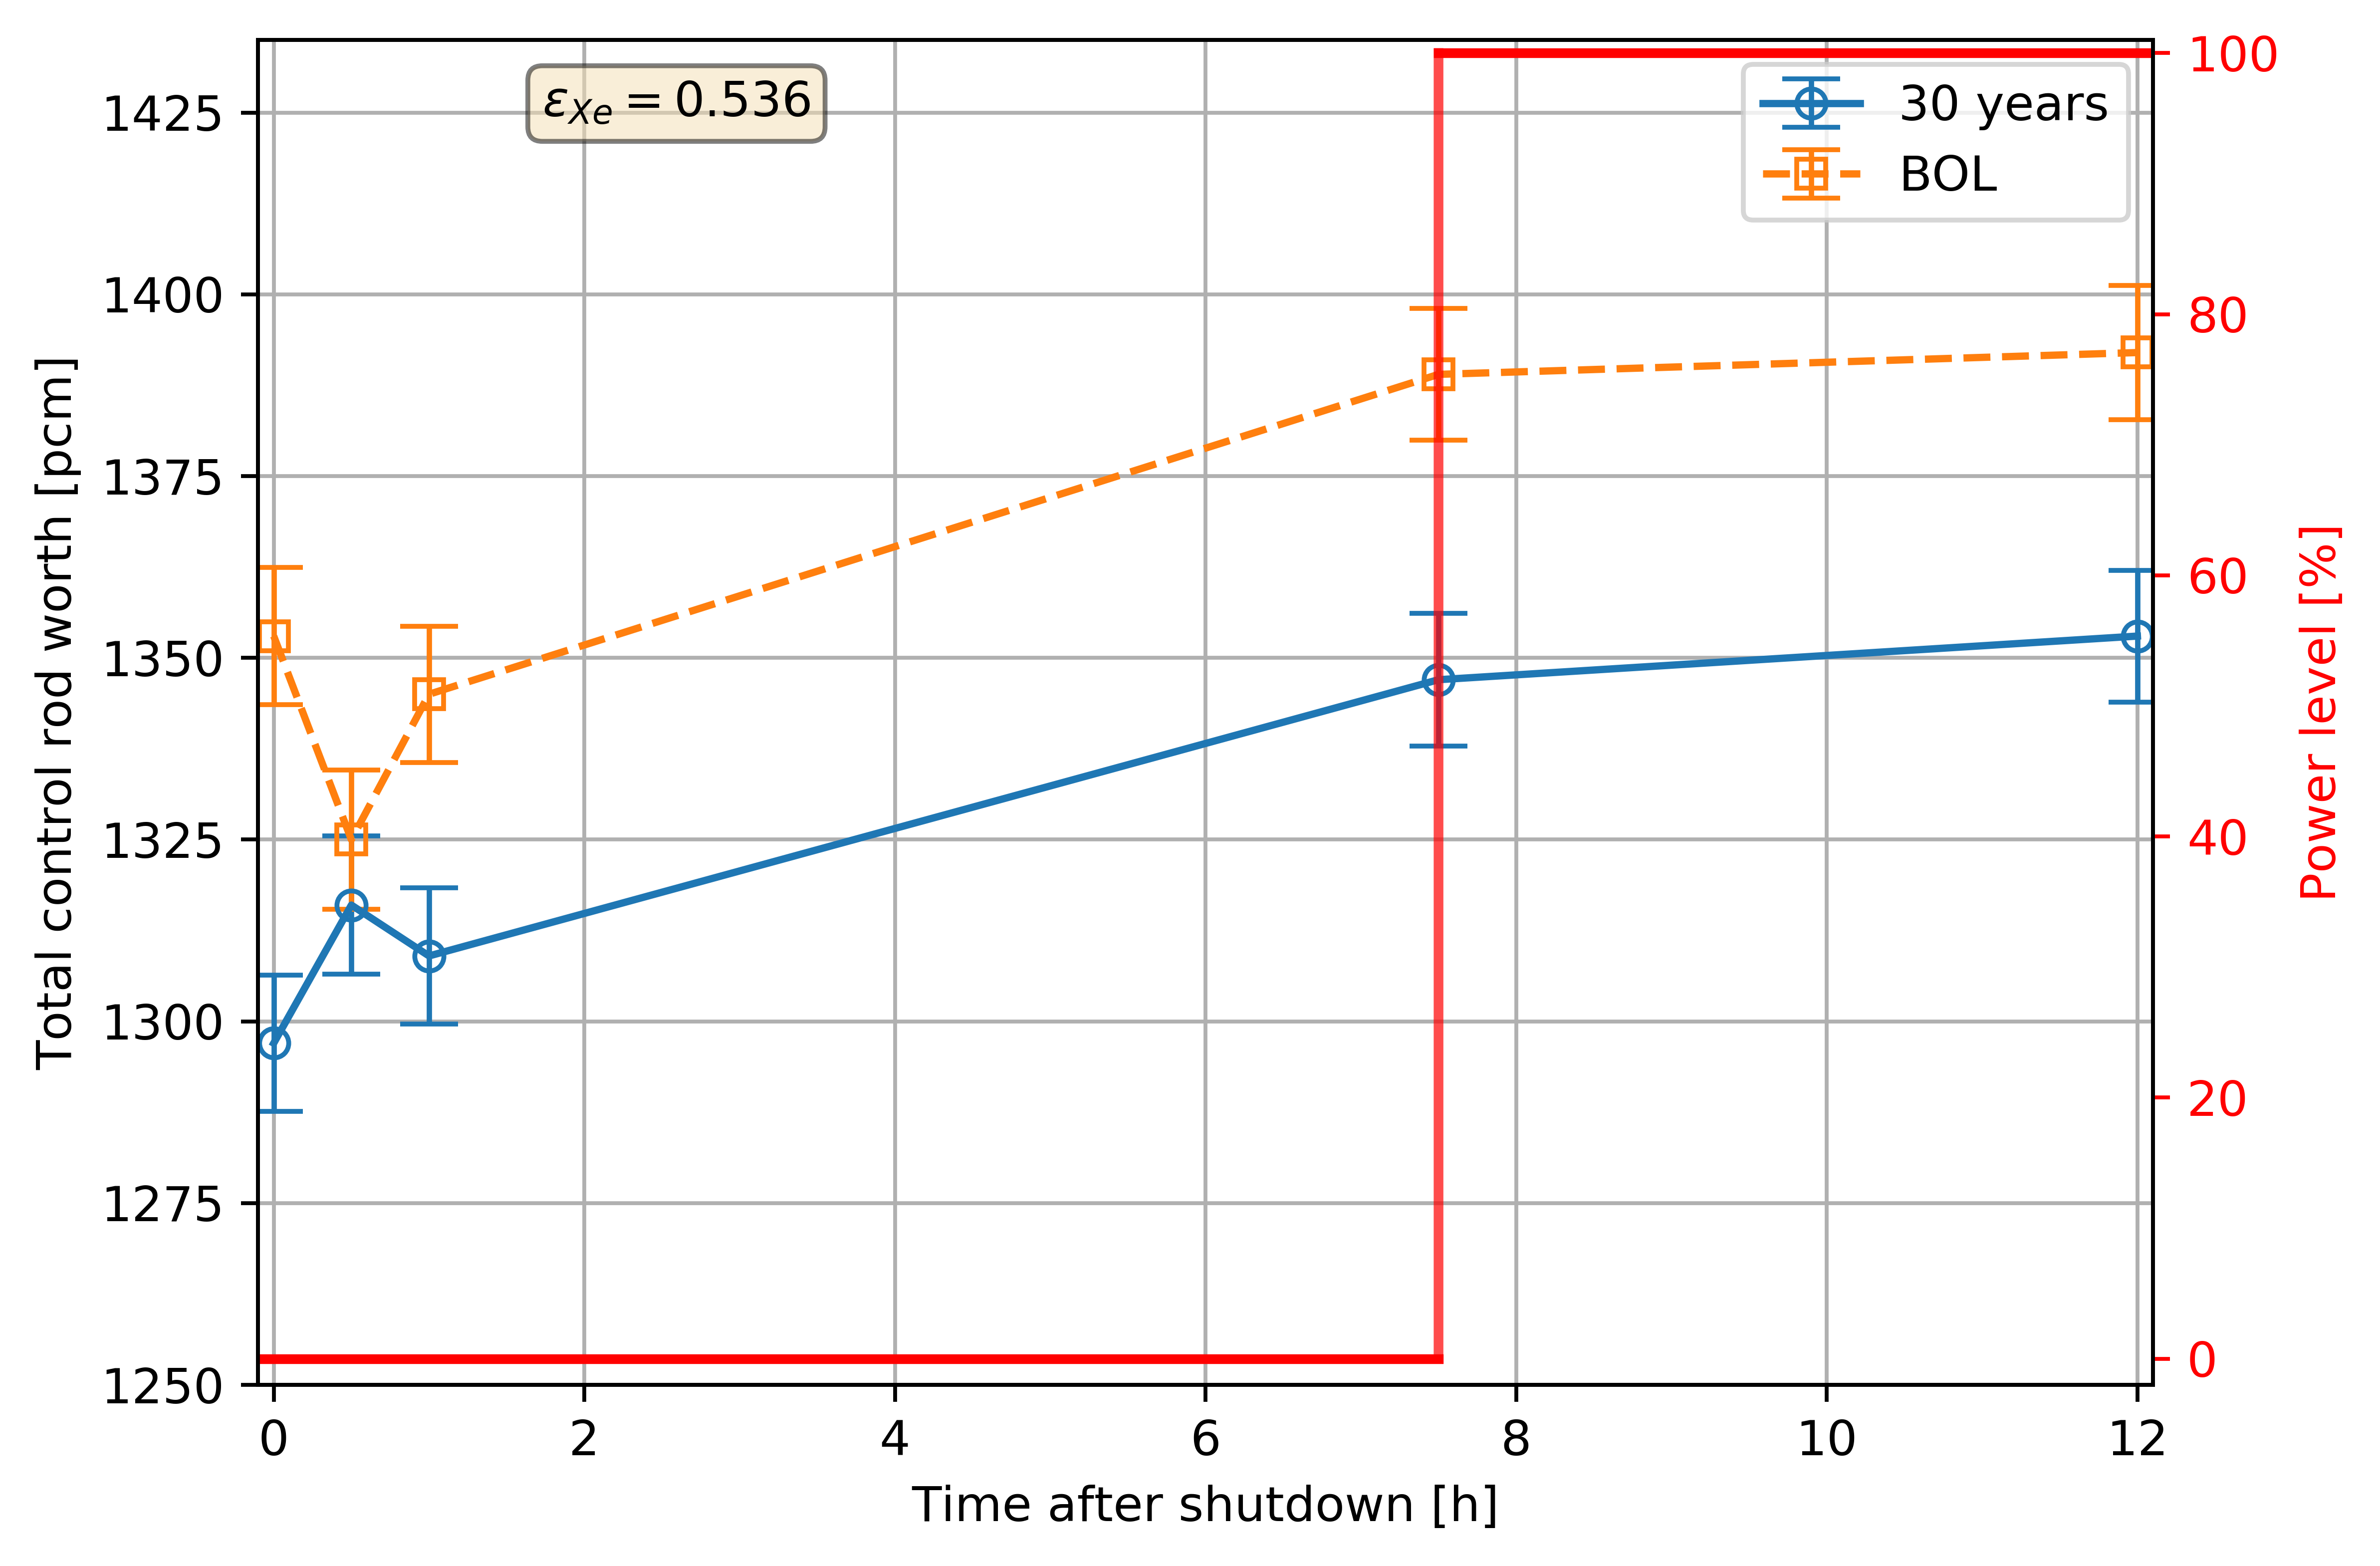
\includegraphics[width=0.95\textwidth]{ch6/saf_par/crw_evo_kl25.png}\\
	\vspace{-10mm}
	\hspace{+0.05mm}
	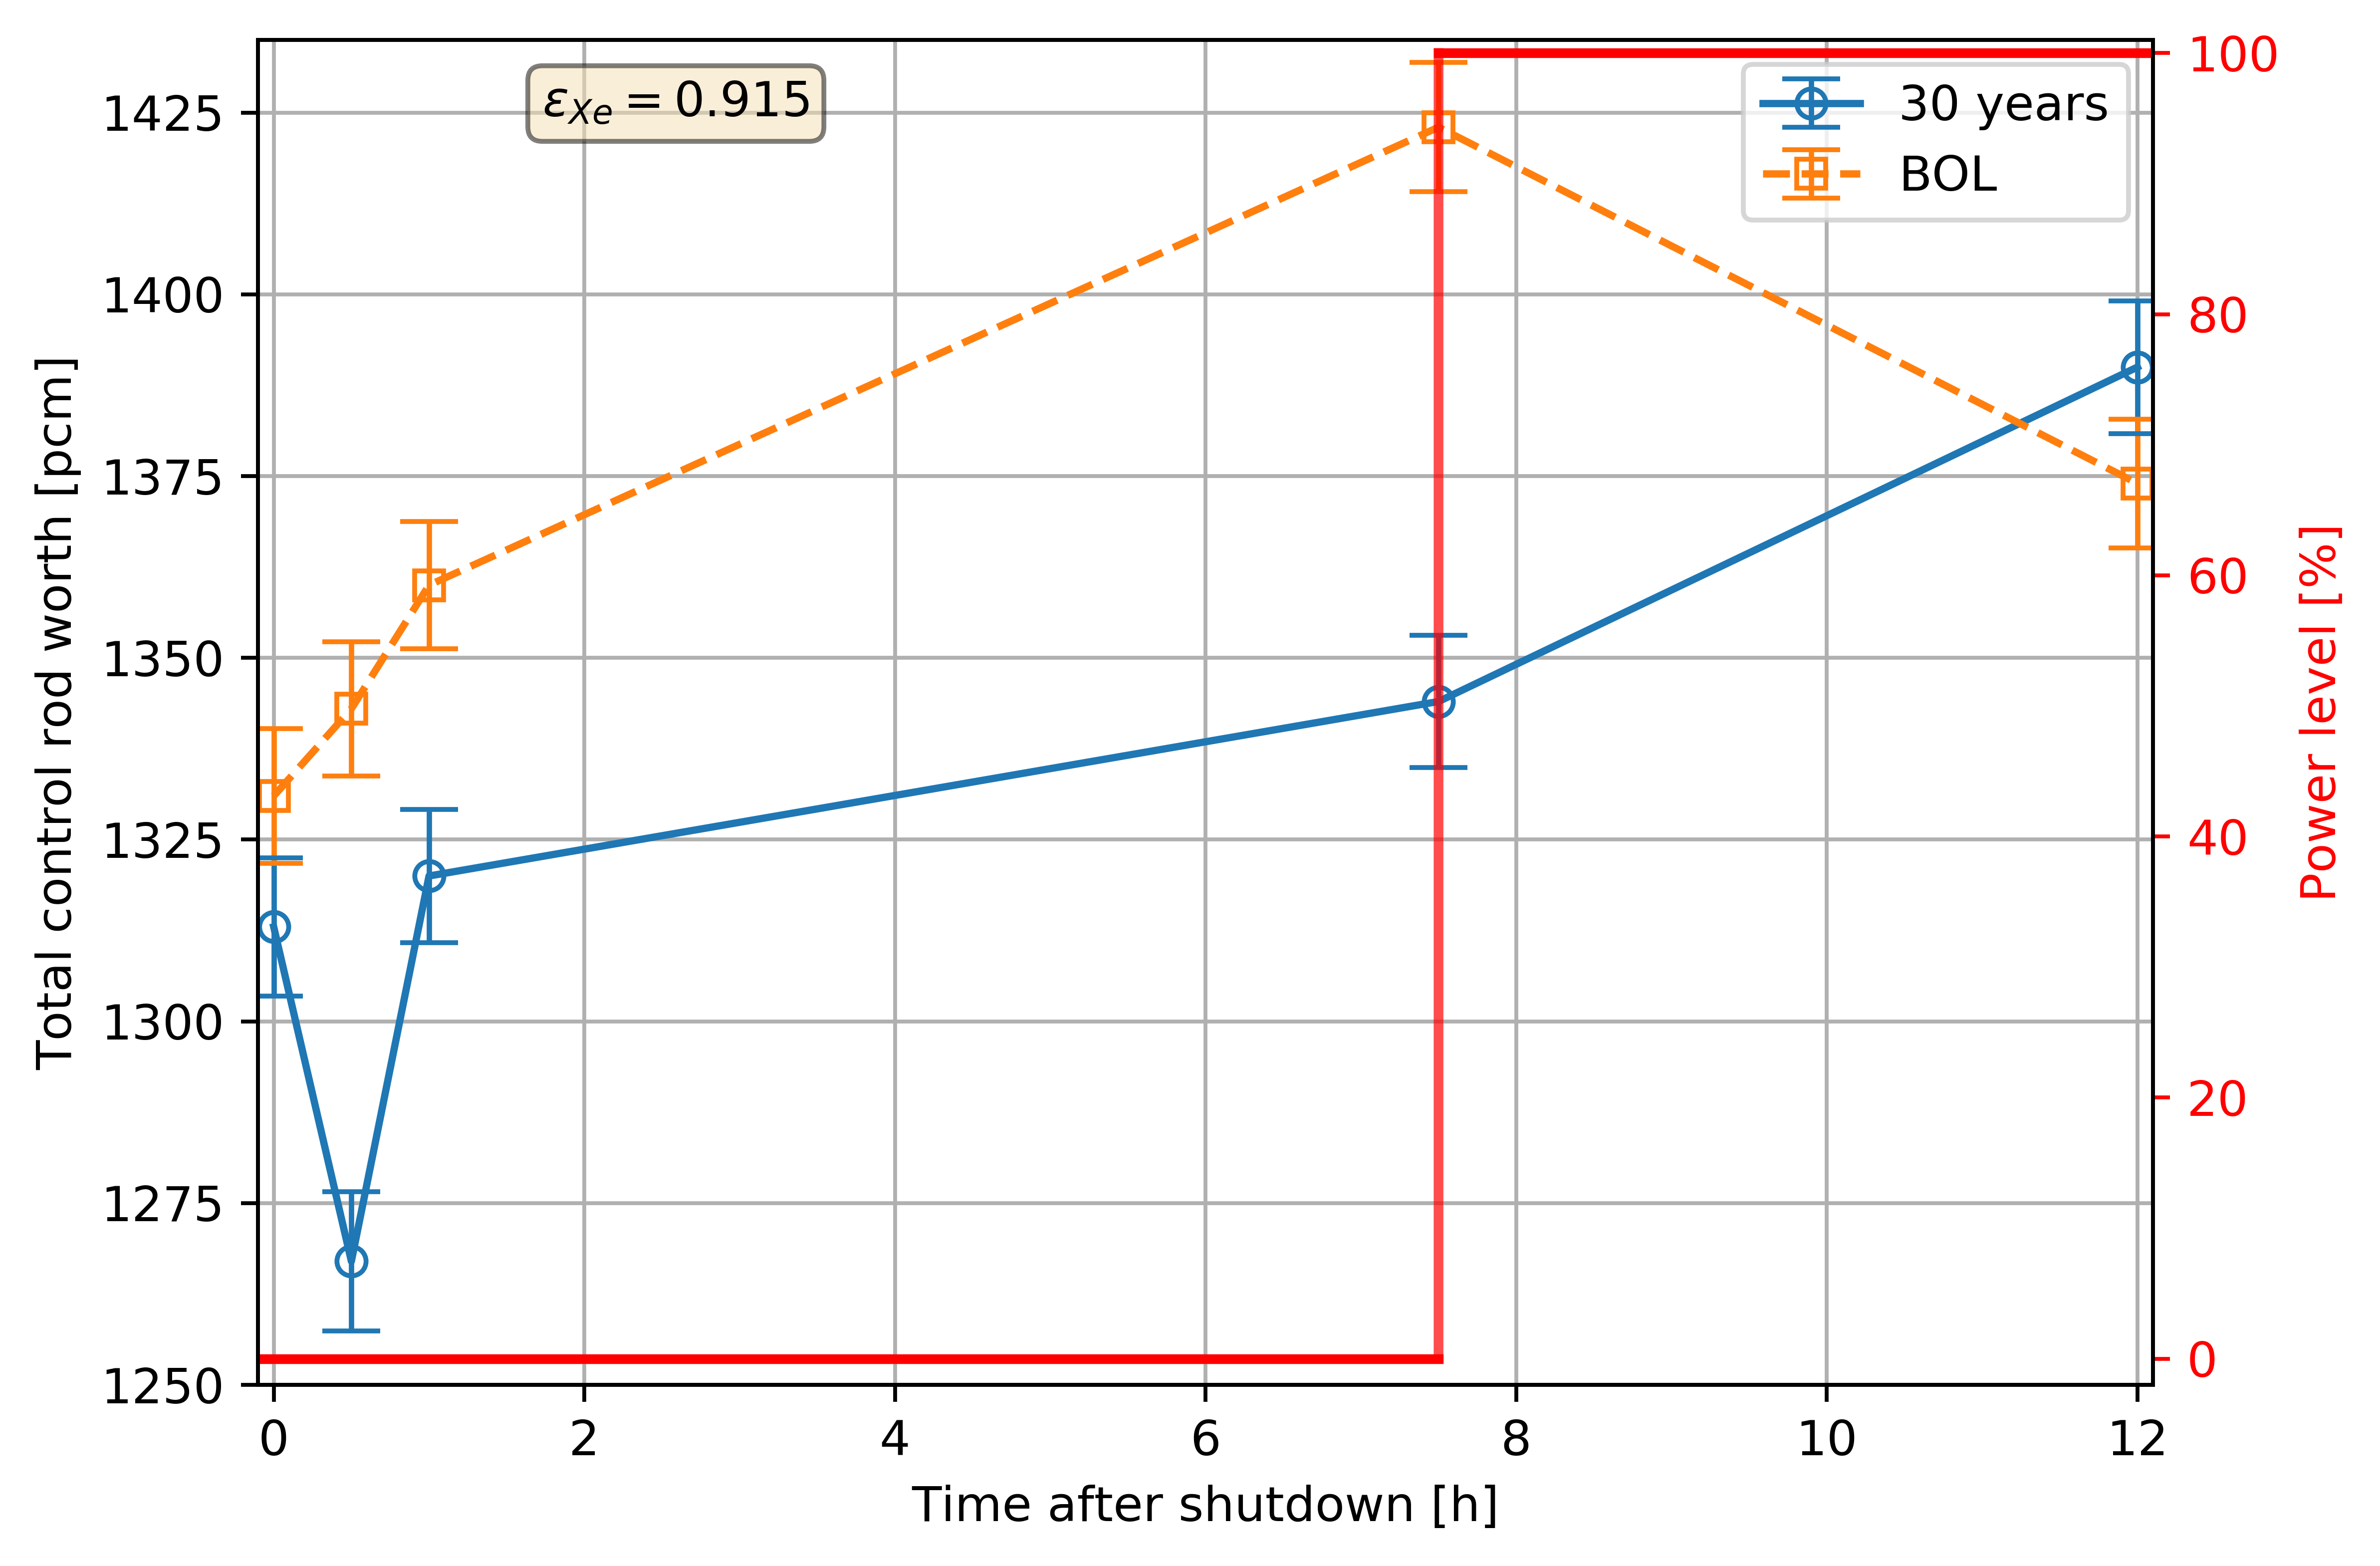
\includegraphics[width=0.95\textwidth]{ch6/saf_par/crw_evo_kl100.png}
	\vspace{-3mm}
	\caption{with moderate (upper) and high (lower) removal efficiency. The 
		uncertainty $\pm\sigma$ region is shaded.}
	\label{fig:msbr-lf-crw-evo}
\end{figure}

\section{Concluding remarks}